\documentclass[a4paper]{report}

\usepackage{xcolor}
\usepackage{sectsty}
\usepackage{setspace}
\usepackage{parskip}
\usepackage[titletoc]{appendix}% http://ctan.org/pkg/appendices
\usepackage{abstract}

\newcommand{\mypapersize}{A4}
\renewcommand{\baselinestretch}{1.3}
\newcommand{\mylaterality}{oneside}
\newcommand{\myparskip}{half}
\newcommand{\myfontsize}{12pt}
\newcommand{\mylinespread}{1.0}
\newcommand{\mydispositioncolor}{30,103,182}
\newcommand{\mycolorlinks}{true}

%%%% Time-stamp: <2015-08-22 17:20:32 vk>
%%%% === Disclaimer: =======================================================
%% created by
%%
%%      Karl Voit
%%
%% using GNU/Linux, GNU Emacs & LaTeX 2e
%%
%doc%
%doc% \section{\texttt{typographic\_settings.tex} --- Typographic finetuning}
%doc%
%doc% The settings of file \verb#template/typographic_settings.tex# contain
%doc% typographic finetuning related to things mentioned in literature.  The
%doc% settings in this file relates to personal taste and most of all: 
%doc% \emph{typographic experience}. 
%doc% 
%doc% \paragraph{What should I do with this file?} You might as well skip the whole
%doc% file by excluding the \verb#\input{template/typographic_settings.tex}# command
%doc% in \texttt{main.tex}.  For standard usage it is recommended to stay with the
%doc% default settings.
%doc% 
%doc% 
%% ========================================================================

%doc%
%doc% Some basic microtypographic settings are provided by the
%doc% \texttt{microtype}
%doc% package\footnote{\url{http://ctan.org/pkg/microtype}}. This template
%doc% uses the rather conservative package parameters: \texttt{protrusion=true,factor=900}.

\usepackage[protrusion=true,factor=900]{microtype}



%doc%
%doc% \subsection{French spacing}
%doc%
%doc% \paragraph{Why?} see~\textcite[p.\,28, p.\,30]{Bringhurst1993}: `2.1.4 Use a single word space between sentences.'
%doc%
%doc% \paragraph{How?} see~\textcite[p.\,185]{Eijkhout2008}:\\
%doc% \verb#\frenchspacing  %% Macro to switch off extra space after punctuation.# \\
\frenchspacing  %% Macro to switch off extra space after punctuation.
%doc%
%doc% Note: This setting might be default for \myacro{KOMA} script.
%doc%


%doc%
%doc% \subsection{Font}
%doc% 
%doc% This template is using the Palatino font (package \texttt{mathpazo}) which results
%doc% in a legible document and matching mathematical fonts for printout.
%doc% 
%doc% It is highly recommended that you either stick to the Palatino font or use the
%doc% \LaTeX{} default fonts (by removing the package \texttt{mathpazo}).
%doc% 
%doc% Chosing different fonts is not
%doc% an easy task. Please leave this to people with good knowledge on this subject.
%doc% 
%doc% One valid reason to change the default fonts is when your document is mainly
%doc% read on a computer screen. In this case it is recommended to switch to a font
%doc% \textsf{which is sans-serif like this}. This template contains several alternative
%doc% font packages which can be activated in this file.
%doc% 

% for changing the default font, please go to the next subsection!

%doc%
%doc% \subsection{Text figures}
%doc% 
%doc% \ldots also called old style numbers such as 0123456789. 
%doc% (German: \enquote{Mediäval\-ziffern\footnote{\url{https://secure.wikimedia.org/wikibooks/de/wiki/LaTeX-W\%C3\%B6rterbuch:\_Medi\%C3\%A4valziffern}}})
%doc% \paragraph{Why?} see~\textcite[p.\,44f]{Bringhurst1993}: 
%doc% \begin{quote}
%doc% `3.2.1 If the font includes both text figures and titling figures, use
%doc%  titling figures only with full caps, and text figures in all other
%doc%  circumstances.'
%doc% \end{quote}
%doc% 
%doc% \paragraph{How?} 
%doc% Quoted from Wikibooks\footnote{\url{https://secure.wikimedia.org/wikibooks/en/wiki/LaTeX/Formatting\#Text\_figures\_.28.22old\_style.22\_numerals.29}}:
%doc% \begin{quote}
%doc% Some fonts do not have text figures built in; the textcomp package attempts to
%doc% remedy this by effectively generating text figures from the currently-selected
%doc% font. Put \verb#\usepackage{textcomp}# in your preamble. textcomp also allows you to
%doc% use decimal points, properly formatted dollar signs, etc. within
%doc% \verb#\oldstylenums{}#.
%doc% \end{quote}
%doc% \ldots but proposed \LaTeX{} method does not work out well. Instead use:\\
%doc% \verb#\usepackage{hfoldsty}#  (enables text figures using additional font) or \\
%doc% \verb#\usepackage[sc,osf]{mathpazo}# (switches to Palatino font with small caps and old style figures enabled).
%doc%
%\usepackage{hfoldsty}  %% enables text figures using additional font
%% ... OR use ...
\usepackage[sc,osf]{mathpazo} %% switches to Palatino with small caps and old style figures

%% Font selection from:
%%     http://www.matthiaspospiech.de/latex/vorlagen/allgemein/preambel/fonts/
%% use following lines *instead* of the mathpazo package above:
%% ===== Serif =========================================================
%% for Computer Modern (LaTeX default font), simply remove the mathpazo above
%\usepackage{charter}\linespread{1.05} %% Charter
%\usepackage{bookman}                  %% Bookman (laedt Avant Garde !!)
%\usepackage{newcent}                  %% New Century Schoolbook (laedt Avant Garde !!)
%% ===== Sans Serif ====================================================
%\renewcommand{\familydefault}{\sfdefault}  %% this one in *combination* with the default mathpazo package
%\usepackage{cmbright}                  %% CM-Bright (eigntlich eine Familie)
%\usepackage{tpslifonts}                %% tpslifonts % Font for Slides


%doc% 
%doc% \subsection{\texttt{myacro} --- Abbrevations using \textsc{small caps}}\myinteresting
%doc% \label{sec:myacro}
%doc% 
%doc% \paragraph{Why?} see~\textcite[p.\,45f]{Bringhurst1993}: `3.2.2 For abbrevations and
%doc% acronyms in the midst of normal text, use spaced small caps.'
%doc% 
%doc% \paragraph{How?} Using the predefined macro \verb#\myacro{}# for things like
%doc% \myacro{UNO} or \myacro{UNESCO} using \verb#\myacro{UNO}# or \verb#\myacro{UNESCO}#.
%doc% 
\DeclareRobustCommand{\myacro}[1]{\textsc{\lowercase{#1}}} %%  abbrevations using small caps


%doc% 
%doc% \subsection{Colorized headings and links}
%doc% 
%doc% This document template is able to generate an output that uses colorized
%doc% headings, captions, page numbers, and links. The color named `DispositionColor'
%doc% used in this document is defined near the definition of package \texttt{color}
%doc% in the preamble (see section~\ref{subsec:miscpackages}). The changes required
%doc% for headings, page numbers, and captions are defined here.
%doc% 
%doc% Settings for colored links are handled by the definitions of the
%doc% \texttt{hyperref} package (see section~\ref{sec:pdf}).
%doc% 
\definecolor{DispositionColor}{RGB}{30,103,182}
\definecolor{chocolate(web)}{RGB}{191,76,58}
\definecolor{cerise}{RGB}{232,156,57}

\chapterfont{\color{DispositionColor}}
\sectionfont{\color{DispositionColor}}
\subsectionfont{\color{chocolate(web)}}
\subsubsectionfont{\color{cerise}}
\paragraphfont{\color{DispositionColor}}


%\setheadsepline{.4pt}[\color{DispositionColor}]
%\renewcommand{\headfont}{\normalfont\sffamily\color{DispositionColor}}
%\renewcommand{\pnumfont}{\normalfont\sffamily\color{DispositionColor}}
%\addtokomafont{disposition}{\color{DispositionColor}}
%\addtokomafont{caption}{\color{DispositionColor}\footnotesize}
%\addtokomafont{captionlabel}{\color{DispositionColor}}



%doc% 
%doc% \subsection{No figures or tables below footnotes}
%doc% 
%doc% \LaTeX{} places floating environments below footnotes if \texttt{b}
%doc% (bottom) is used as (default) placement algorithm. This is certainly
%doc% not appealing for most people and is deactivated in this template by
%doc% using the package \texttt{footmisc} with its option \texttt{bottom}.
%doc% 
%% see also: http://www.komascript.de/node/858 (German description)
\usepackage[bottom]{footmisc}

%doc% 
%doc% \subsection{Spacings of list environments}
%doc% 
%doc% By default, \LaTeX{} is using vertical spaces between items of enumerate, 
%doc% itemize and description environments. This is fine for multi-line items.
%doc% Many times, the user does just write single-line items where the larger
%doc% vertical space is inappropriate. The \href{http://ctan.org/pkg/enumitem}{enumitem}
%doc% package provides replacements for the pre-defined list environments and
%doc% offers many options to modify their appearances.
%doc% This template is using the package option for \texttt{noitemsep} which
%doc% mimimizes the vertical space between list items.
%doc% 
\usepackage{enumitem}
\setlist{noitemsep} %% kills the space between items



\makeatletter
\newcommand*{\addFileDependency}[1]{% argument=file name and extension
  \typeout{(#1)}
  \@addtofilelist{#1}
  \IfFileExists{#1}{}{\typeout{No file #1.}}
}
\makeatother

\newcommand*{\myexternaldocument}[1]{%
  \externaldocument{#1}%
  \addFileDependency{#1.tex}%
  \addFileDependency{#1.aux}%
}



% Fix the abstract vertical space 
\renewcommand{\abstractnamefont}{\normalfont\Large\bfseries\color{DispositionColor}}
\setlength{\abstitleskip}{1cm}

% default style for itemize
\setlist[itemize]{label=\textbullet}


% Bold and blue 

\newcommand{\bb}[1]{\textbf{#1}}

%doc% 
%doc% \subsection{\texttt{csquotes} --- Correct quotation marks}\myinteresting
%doc% \label{sub:csquotes}
%doc% 
%doc% \emph{Never} use quotation marks found on your keyboard.
%doc% They end up in strange characters or false looking quotation marks.
%doc% 
%doc% In \LaTeX{} you are able to use typographically correct quotation marks. The package 
%doc% \href{http://www.ctan.org/pkg/csquotes}{\texttt{csquotes}} offers you with 
%doc% \verb#\enquote{foobar}# a command to get correct quotation marks around \enquote{foobar}.
%doc% Please do check the package options in order to modify
%doc% its settings according to the language used\footnote{most of the time in 
%doc% combination with the language set in the options of the \texttt{babel} package}.
%doc% 
%doc% \href{http://www.ctan.org/pkg/csquotes}{\texttt{csquotes}} is also recommended 
%doc% by \texttt{biblatex} (see Section~\ref{sec:references}). 
%\usepackage[babel=true,strict=true,english=american,german=guillemets]{csquotes}

%doc% 
%doc% \subsection{Line spread}
%doc% 
%doc% If you have to enlarge the distance between two lines of text, you can
%doc% increase it using the \texttt{\mylinespread} command in \texttt{main.tex}. By default, it is
%doc% deactivated (set to 100~percent). Modify only with caution since it influences the
%doc% page layout and could lead to ugly looking documents.
\linespread{\mylinespread}

%doc% 
%doc% \subsection{Optional: Lines above and below the chapter head}
%doc% 
%doc% This is not quite something typographic but rather a matter of taste.
%doc% \myacro{KOMA} Script offers \href{http://www.komascript.de/node/24}{a method to
%doc% add lines above and below chapter head} which is disabled by
%doc% default. If you want to enable this feature, remove corresponding
%doc% comment characters from the settings.
%doc% 
%% Source: http://www.komascript.de/node/24
%disabled% %% 1st get a new command
%disabled% \newcommand*{\ORIGchapterheadstartvskip}{}%
%disabled% %% 2nd save the original definition to the new command
%disabled% \let\ORIGchapterheadstartvskip=\chapterheadstartvskip
%disabled% %% 3rd redefine the command using the saved original command
%disabled% \renewcommand*{\chapterheadstartvskip}{%
%disabled%   \ORIGchapterheadstartvskip
%disabled%   {%
%disabled%     \setlength{\parskip}{0pt}%
%disabled%     \noindent\color{DispositionColor}\rule[.3\baselineskip]{\linewidth}{1pt}\par
%disabled%   }%
%disabled% }
%disabled% %% see above
%disabled% \newcommand*{\ORIGchapterheadendvskip}{}%
%disabled% \let\ORIGchapterheadendvskip=\chapterheadendvskip
%disabled% \renewcommand*{\chapterheadendvskip}{%
%disabled%   {%
%disabled%     \setlength{\parskip}{0pt}%
%disabled%     \noindent\color{DispositionColor}\rule[.3\baselineskip]{\linewidth}{1pt}\par
%disabled%   }%
%disabled%   \ORIGchapterheadendvskip
%disabled% }

%doc% 
%doc% \subsection{Optional: Chapter thumbs}
%doc% 
%doc% This is not quite something typographic but rather a matter of taste.
%doc% \myacro{KOMA} Script offers \href{http://www.komascript.de/chapterthumbs-example}{a method to
%doc% add chapter thumbs} (in combination with the package \texttt{scrpage2}) which is disabled by
%doc% default. If you want to enable this feature, remove corresponding
%doc% comment characters from the settings.
%doc% 
%disabled% \makeatletter
%disabled% % Safty first
%disabled% \@ifundefined{chapter}{\let\chapter\undefined
%disabled%   \chapter must be defined to use chapter thumbs!}{%
%disabled%  
%disabled% % Two new commands for the width and height of the boxes with the
%disabled% % chapter number at the thumbs (use of commands instead of lengths
%disabled% % for sparing registers)
%disabled% \newcommand*{\chapterthumbwidth}{2em}
%disabled% \newcommand*{\chapterthumbheight}{1em}
%disabled%  
%disabled% % Two new commands for the colors of the box background and the
%disabled% % chapter numbers of the thumbs
%disabled% \newcommand*{\chapterthumbboxcolor}{black}
%disabled% \newcommand*{\chapterthumbtextcolor}{white}
%disabled%  
%disabled% % New command to set a chapter thumb. I'm using a group at this
%disabled% % command, because I'm changing the temporary dimension \@tempdima
%disabled% \newcommand*{\putchapterthumb}{%
%disabled%   \begingroup
%disabled%     \Large
%disabled%     % calculate the horizontal possition of the right paper border
%disabled%     % (I ignore \hoffset, because I interprete \hoffset moves the page
%disabled%     % at the paper e.g. if you are using cropmarks)
%disabled%     \setlength{\@tempdima}{\@oddheadshift}% (internal from scrpage2)
%disabled%     \setlength{\@tempdima}{-\@tempdima}%
%disabled%     \addtolength{\@tempdima}{\paperwidth}%
%disabled%     \addtolength{\@tempdima}{-\oddsidemargin}%
%disabled%     \addtolength{\@tempdima}{-1in}%
%disabled%     % putting the thumbs should not change the horizontal
%disabled%     % possition
%disabled%     \rlap{%
%disabled%       % move to the calculated horizontal possition
%disabled%       \hspace*{\@tempdima}%
%disabled%       % putting the thumbs should not change the vertical
%disabled%       % possition
%disabled%       \vbox to 0pt{%
%disabled%         % calculate the vertical possition of the thumbs (I ignore
%disabled%         % \voffset for the same reasons told above)
%disabled%         \setlength{\@tempdima}{\chapterthumbwidth}%
%disabled%         \multiply\@tempdima by\value{chapter}%
%disabled%         \addtolength{\@tempdima}{-\chapterthumbwidth}%
%disabled%         \addtolength{\@tempdima}{-\baselineskip}%
%disabled%         % move to the calculated vertical possition
%disabled%         \vspace*{\@tempdima}%
%disabled%         % put the thumbs left so the current horizontal possition
%disabled%         \llap{%
%disabled%           % and rotate them
%disabled%           \rotatebox{90}{\colorbox{\chapterthumbboxcolor}{%
%disabled%               \parbox[c][\chapterthumbheight][c]{\chapterthumbwidth}{%
%disabled%                 \centering
%disabled%                 \textcolor{\chapterthumbtextcolor}{%
%disabled%                   \strut\thechapter}\\
%disabled%               }%
%disabled%             }%
%disabled%           }%
%disabled%         }%
%disabled%         % avoid overfull \vbox messages
%disabled%         \vss
%disabled%       }%
%disabled%     }%
%disabled%   \endgroup
%disabled% }
%disabled%  
%disabled% % New command, which works like \lohead but also puts the thumbs (you
%disabled% % cannot use \ihead with this definition but you may change this, if
%disabled% % you use more internal scrpage2 commands)
%disabled% \newcommand*{\loheadwithchapterthumbs}[2][]{%
%disabled%   \lohead[\putchapterthumb#1]{\putchapterthumb#2}%
%disabled% }
%disabled%  
%disabled% % initial use
%disabled% \loheadwithchapterthumbs{}
%disabled% \pagestyle{scrheadings}
%disabled%  
%disabled% }
%disabled% \makeatother

%%%% END
%%% Local Variables:
%%% mode: latex
%%% mode: auto-fill
%%% mode: flyspell
%%% eval: (ispell-change-dictionary "en_US")
%%% TeX-master: "../main"
%%% End:
%% vim:foldmethod=expr
%% vim:fde=getline(v\:lnum)=~'^%%%%'?0\:getline(v\:lnum)=~'^%doc.*\ .\\%(sub\\)\\?section{.\\+'?'>1'\:'1':

%% Time-stamp: <2015-04-30 17:19:58 vk>
%%%% === Disclaimer: =======================================================
%% created by
%%
%%      Karl Voit
%%
%% using GNU/Linux, GNU Emacs & LaTeX 2e
%%

%doc%
%doc% \section{\texttt{mycommands.tex} --- various definitions}\myinteresting
%doc% \label{sec:mycommands}
%doc%
%doc% In file \verb#template/mycommands.tex# many useful commands are being
%doc% defined. 
%doc% 
%doc% \paragraph{What should I do with this file?} Please take a look at its 
%doc% content to get the most out of your document.
%doc% 

%doc% 
%doc% One of the best advantages of \LaTeX{} compared to \myacro{WYSIWYG} software products is
%doc% the possibility to define and use macros within text. This empowers the user to
%doc% a great extend.  Many things can be defined using \verb#\newcommand{}# and
%doc% automates repeating tasks. It is recommended to use macros not only for
%doc% repetitive tasks but also for separating form from content such as \myacro{CSS}
%doc% does for \myacro{XHTML}. Think of including graphics in your document: after
%doc% writing your book, you might want to change all captions to the upper side of
%doc% each figure. In this case you either have to modify all
%doc% \texttt{includegraphics} commands or you were clever enough to define something
%doc% like \verb#\myfig#\footnote{See below for a detailed description}. Using a
%doc% macro for including graphics enables you to modify the position caption on only
%doc% \emph{one} place: at the definition of the macro.
%doc% 
%doc% The following section describes some macros that came with this document template
%doc% from \myLaT and you are welcome to modify or extend them or to create
%doc% your own macros!
%doc% 

%doc% 
%doc% \subsection{\texttt{myfig} --- including graphics made easy}
%doc% 
%doc% The classic: you can easily add graphics to your document with \verb#\myfig#:
%doc% \begin{verbatim}
%doc%  \myfig{flower}%% filename w/o extension in the folder figures
%doc%        {width=0.7\textwidth}%% maximum width/height, aspect ratio will be kept
%doc%        {This flower was photographed at my home town in 2010}%% caption
%doc%        {Home town flower}%% optional (short) caption for list of figures
%doc%        {fig:flower}%% label
%doc% \end{verbatim}
%doc% 
%doc% There are many advantages of this command (compared to manual
%doc% \texttt{figure} environments and \texttt{includegraphics} commands:
%doc% \begin{itemize}
%doc% \item consistent style throughout the whole document
%doc% \item easy to change; for example move caption on top
%doc% \item much less characters to type (faster, error prone)
%doc% \item less visual clutter in the \TeX{}-files
%doc% \end{itemize}
%doc% 
%doc% 
\newcommand{\myfig}[5]{
%% example:
% \myfig{}%% filename in figures folder
%       {width=0.5\textwidth,height=0.5\textheight}%% maximum width/height, aspect ratio will be kept
%       {}%% caption
%       {}%% optional (short) caption for list of figures
%       {}%% label
\begin{figure}%[htp]
  \centering
  \includegraphics[keepaspectratio,#2]{figures/#1}
  \caption[#4]{#3}
  \label{#5} %% NOTE: always label *after* caption!
\end{figure}
}


%doc% 
%doc% \subsection{\texttt{myclone} --- repeat things!}
%doc% 
%doc% Using \verb#\myclone[42]{foobar}# results the text \enquote{foobar} printed 42 times.
%doc% But you can not only repeat text output with \texttt{myclone}. 
%doc%
%doc% Default argument
%doc% for the optional parameter \enquote{number of times} (like \enquote{42} in the example above) 
%doc% is set to two.
%doc% 
%% \myclone[x]{text}
\newcounter{myclonecnt}
\newcommand{\myclone}[2][2]{%
  \setcounter{myclonecnt}{#1}%
  \whiledo{\value{myclonecnt}>0}{#2\addtocounter{myclonecnt}{-1}}%
}

%old% %d oc% 
%old% %d oc% \subsection{\texttt{fixxme} --- sidemark something as unfinished}
%old% %d oc% 
%old% %d oc% You know it: something has to be fixed and you can not do it right
%old% %d oc% now. In order to \texttt{not} forget about it, you might want to add a
%old% %d oc% note like \verb+\fixxme{check again}+ which inserts a note on the page
%old% %d oc% margin such as this\fixxme{check again} example.
%old% %d oc%
%old% \newcommand{\fixxme}[1]{%%
%old% \textcolor{red}{FIXXME}\marginpar{\textcolor{red}{#1}}%%
%old% }


%%%% End 
%%% Local Variables:
%%% mode: latex
%%% mode: auto-fill
%%% mode: flyspell
%%% eval: (ispell-change-dictionary "en_US")
%%% TeX-master: "../main"
%%% End:
%% vim:foldmethod=expr
%% vim:fde=getline(v\:lnum)=~'^%%%%'?0\:getline(v\:lnum)=~'^%doc.*\ .\\%(sub\\)\\?section{.\\+'?'>1'\:'1':

%%%% Time-stamp: <2018-03-11 14:31:45 vk>
%%%% === Disclaimer: =======================================================
%% created by
%%
%%      Karl Voit
%%
%% using GNU/Linux, GNU Emacs & LaTeX 2e
%%

%doc%
%doc% \section{\texttt{pdf\_settings.tex} --- Settings related to PDF output}
%doc% \label{sec:pdf}
%doc%
%doc% The file \verb#template/pdf_settings.tex# basically contains the definitions for
%doc% the \href{http://tug.org/applications/hyperref/}{\texttt{hyperref} package}
%doc% including the
%doc% \href{http://www.ctan.org/tex-archive/macros/latex/required/graphics/}{\texttt{graphicx}
%doc% package}. Since these settings should be the last things of any \LaTeX{}
%doc% preamble, they got their own \TeX{} file which is included in \texttt{main.tex}.
%doc%
%doc% \paragraph{What should I do with this file?} The settings in this file are
%doc% important for \myacro{PDF} output and including graphics. Do not exclude the
%doc% related \texttt{input} command in \texttt{main.tex}. But you might want to
%doc% modify some settings after you read the
%doc% \href{http://tug.org/applications/hyperref/}{documentation of the \texttt{hyperref} package}.
%doc%


%% Fix positioning of images in PDF viewers. (disabled by
%% default; see https://github.com/novoid/LaTeX-KOMA-template/issues/4
%% for more information)
%% I do not have time to read about possible side-effect of this
%% package for now.
% \usepackage[hypcap]{caption}

%% Declarations of hyperref should be the last definitions of the preamble:
%% FIXXME: black-and-white-version for printing!

\pdfcompresslevel=9

\usepackage[%
unicode=true, % loads with unicode support
%a4paper=true, %
%pdftex=true, %
backref, %
pagebackref=false, % creates backward references too
bookmarks=true, % generate bookmarks in PDF files
bookmarksopen=false, % when starting with AcrobatReader, the Bookmarkcolumn is opened
pdfpagemode=UseNone,% None, UseOutlines, UseThumbs, FullScreen
plainpages=false, % correct, if pdflatex complains: ``destination with same identifier already exists''
%% colors: https://secure.wikimedia.org/wikibooks/en/wiki/LaTeX/Colors
urlcolor=DispositionColor, %%
linkcolor=DispositionColor, %%
%pagecolor=DispositionColor, %%
citecolor=DispositionColor, %%
anchorcolor=DispositionColor, %%
colorlinks=\mycolorlinks, % turn on/off colored links (on: better for
                          % on-screen reading; off: better for printout versions)
]{hyperref}

%% all strings need to be loaded after hyperref was loaded with unicode support
%% if not the field is garbled in the output for characters like ČŽĆŠĐ
%\hypersetup{
%pdftitle={\mytitle}, %
%pdfauthor={\myauthor}, %
%pdfsubject={\mysubject}, %
%pdfcreator={Accomplished with: pdfLaTeX, biber, and hyperref-package. No animals, MS-EULA or BSA-rules were harmed.},
%pdfproducer={\myauthor},
%pdfkeywords={\mykeywords}
%}

%\DeclareGraphicsExtensions{.pdf}

%%%% END
%%% Local Variables:
%%% TeX-master: "../main"
%%% mode: latex
%%% mode: auto-fill
%%% mode: flyspell
%%% eval: (ispell-change-dictionary "en_US")
%%% End:
%% vim:foldmethod=expr
%% vim:fde=getline(v\:lnum)=~'^%%%%'?0\:getline(v\:lnum)=~'^%doc.*\ .\\%(sub\\)\\?section{.\\+'?'>1'\:'1':


\usepackage{float}
\usepackage[T1]{fontenc}
\usepackage[utf8]{inputenc}
\usepackage[french]{babel}
\usepackage{titlesec}
\usepackage{amsmath}

\usepackage{hyperref}
\usepackage{xr-hyper}
\usepackage[nottoc]{tocbibind}

\usepackage{subfig}
\usepackage{graphicx} 
\setlength{\parindent}{1em}
\usepackage[top=0.6in,bottom=0.6in,right=1in,left=1in]{geometry}
\usepackage{graphics}

\usepackage{bookmark} 
\usepackage{caption}
\usepackage[font={color=DispositionColor,bf},figurename=Fig.,labelfont={it}]{caption}

\newcommand\ackname{Remerciements}
\newcommand\abstname{Résumé}

\usepackage[breakable]{tcolorbox}
%\usepackage{parskip} % Stop auto-indenting (to mimic markdown behaviour)

\usepackage{iftex}
\ifPDFTeX
    \usepackage[T1]{fontenc}
    \usepackage{mathpazo}
\else
    \usepackage{fontspec}
\fi

% Maintain compatibility with old templates. Remove in nbconvert 6.0
\let\Oldincludegraphics\includegraphics
% Ensure that by default, figures have no caption (until we provide a
% proper Figure object with a Caption API and a way to capture that
% in the conversion process - todo).

\usepackage{enumerate} % Needed for markdown enumerations to work
\usepackage{textcomp} % defines textquotesingle
% Hack from http://tex.stackexchange.com/a/47451/13684:
\AtBeginDocument{%
    \def\PYZsq{\textquotesingle}% Upright quotes in Pygmentized code
}
\usepackage{upquote} % Upright quotes for verbatim code
\usepackage{eurosym} % defines \euro
\usepackage[mathletters]{ucs} % Extended unicode (utf-8) support
\usepackage{fancyvrb} % verbatim replacement that allows latex
\usepackage{grffile} % extends the file name processing of package graphics 
% to support a larger range
\makeatletter % fix for grffile with XeLaTeX
\def\Gread@@xetex#1{%
    \IfFileExists{"\Gin@base".bb}%
    {\Gread@eps{\Gin@base.bb}}%
    {\Gread@@xetex@aux#1}%
}
\makeatother

% The default LaTeX title has an obnoxious amount of whitespace. By default,
% titling removes some of it. It also provides customization options.
\usepackage{titling}
\usepackage{longtable} % longtable support required by pandoc >1.10
\usepackage{booktabs}  % table support for pandoc > 1.12.2
%\usepackage[inline]{enumitem} % IRkernel/repr support (it uses the enumerate* environment)
\usepackage[normalem]{ulem} % ulem is needed to support strikethroughs (\sout)
% normalem makes italics be italics, not underlines
\usepackage{mathrsfs}

% ANSI colors
\definecolor{ansi-black}{HTML}{3E424D}
\definecolor{ansi-black-intense}{HTML}{282C36}
\definecolor{ansi-red}{HTML}{E75C58}
\definecolor{ansi-red-intense}{HTML}{B22B31}
\definecolor{ansi-green}{HTML}{00A250}
\definecolor{ansi-green-intense}{HTML}{007427}
\definecolor{ansi-yellow}{HTML}{DDB62B}
\definecolor{ansi-yellow-intense}{HTML}{B27D12}
\definecolor{ansi-blue}{HTML}{208FFB}
\definecolor{ansi-blue-intense}{HTML}{0065CA}
\definecolor{ansi-magenta}{HTML}{D160C4}
\definecolor{ansi-magenta-intense}{HTML}{A03196}
\definecolor{ansi-cyan}{HTML}{60C6C8}
\definecolor{ansi-cyan-intense}{HTML}{258F8F}
\definecolor{ansi-white}{HTML}{C5C1B4}
\definecolor{ansi-white-intense}{HTML}{A1A6B2}
\definecolor{ansi-default-inverse-fg}{HTML}{FFFFFF}
\definecolor{ansi-default-inverse-bg}{HTML}{000000}

% commands and environments needed by pandoc snippets
% extracted from the output of `pandoc -s`
\providecommand{\tightlist}{%
    \setlength{\itemsep}{0pt}\setlength{\parskip}{0pt}}
\DefineVerbatimEnvironment{Highlighting}{Verbatim}{commandchars=\\\{\}}
% Add ',fontsize=\small' for more characters per line
\newenvironment{Shaded}{}{}
\newcommand{\KeywordTok}[1]{\textcolor[rgb]{0.00,0.44,0.13}{\textbf{{#1}}}}
\newcommand{\DataTypeTok}[1]{\textcolor[rgb]{0.56,0.13,0.00}{{#1}}}
\newcommand{\DecValTok}[1]{\textcolor[rgb]{0.25,0.63,0.44}{{#1}}}
\newcommand{\BaseNTok}[1]{\textcolor[rgb]{0.25,0.63,0.44}{{#1}}}
\newcommand{\FloatTok}[1]{\textcolor[rgb]{0.25,0.63,0.44}{{#1}}}
\newcommand{\CharTok}[1]{\textcolor[rgb]{0.25,0.44,0.63}{{#1}}}
\newcommand{\StringTok}[1]{\textcolor[rgb]{0.25,0.44,0.63}{{#1}}}
\newcommand{\CommentTok}[1]{\textcolor[rgb]{0.38,0.63,0.69}{\textit{{#1}}}}
\newcommand{\OtherTok}[1]{\textcolor[rgb]{0.00,0.44,0.13}{{#1}}}
\newcommand{\AlertTok}[1]{\textcolor[rgb]{1.00,0.00,0.00}{\textbf{{#1}}}}
\newcommand{\FunctionTok}[1]{\textcolor[rgb]{0.02,0.16,0.49}{{#1}}}
\newcommand{\RegionMarkerTok}[1]{{#1}}
\newcommand{\ErrorTok}[1]{\textcolor[rgb]{1.00,0.00,0.00}{\textbf{{#1}}}}
\newcommand{\NormalTok}[1]{{#1}}

% Additional commands for more recent versions of Pandoc
\newcommand{\ConstantTok}[1]{\textcolor[rgb]{0.53,0.00,0.00}{{#1}}}
\newcommand{\SpecialCharTok}[1]{\textcolor[rgb]{0.25,0.44,0.63}{{#1}}}
\newcommand{\VerbatimStringTok}[1]{\textcolor[rgb]{0.25,0.44,0.63}{{#1}}}
\newcommand{\SpecialStringTok}[1]{\textcolor[rgb]{0.73,0.40,0.53}{{#1}}}
\newcommand{\ImportTok}[1]{{#1}}
\newcommand{\DocumentationTok}[1]{\textcolor[rgb]{0.73,0.13,0.13}{\textit{{#1}}}}
\newcommand{\AnnotationTok}[1]{\textcolor[rgb]{0.38,0.63,0.69}{\textbf{\textit{{#1}}}}}
\newcommand{\CommentVarTok}[1]{\textcolor[rgb]{0.38,0.63,0.69}{\textbf{\textit{{#1}}}}}
\newcommand{\VariableTok}[1]{\textcolor[rgb]{0.10,0.09,0.49}{{#1}}}
\newcommand{\ControlFlowTok}[1]{\textcolor[rgb]{0.00,0.44,0.13}{\textbf{{#1}}}}
\newcommand{\OperatorTok}[1]{\textcolor[rgb]{0.40,0.40,0.40}{{#1}}}
\newcommand{\BuiltInTok}[1]{{#1}}
\newcommand{\ExtensionTok}[1]{{#1}}
\newcommand{\PreprocessorTok}[1]{\textcolor[rgb]{0.74,0.48,0.00}{{#1}}}
\newcommand{\AttributeTok}[1]{\textcolor[rgb]{0.49,0.56,0.16}{{#1}}}
\newcommand{\InformationTok}[1]{\textcolor[rgb]{0.38,0.63,0.69}{\textbf{\textit{{#1}}}}}
\newcommand{\WarningTok}[1]{\textcolor[rgb]{0.38,0.63,0.69}{\textbf{\textit{{#1}}}}}


% Define a nice break command that doesn't care if a line doesn't already
% exist.
\def\br{\hspace*{\fill} \\* }
% Math Jax compatibility definitions
\def\gt{>}
\def\lt{<}
\let\Oldtex\TeX
\let\Oldlatex\LaTeX
\renewcommand{\TeX}{\textrm{\Oldtex}}
\renewcommand{\LaTeX}{\textrm{\Oldlatex}}




% Pygments definitions
\makeatletter
\def\PY@reset{\let\PY@it=\relax \let\PY@bf=\relax%
    \let\PY@ul=\relax \let\PY@tc=\relax%
    \let\PY@bc=\relax \let\PY@ff=\relax}
\def\PY@tok#1{\csname PY@tok@#1\endcsname}
\def\PY@toks#1+{\ifx\relax#1\empty\else%
    \PY@tok{#1}\expandafter\PY@toks\fi}
\def\PY@do#1{\PY@bc{\PY@tc{\PY@ul{%
                \PY@it{\PY@bf{\PY@ff{#1}}}}}}}
\def\PY#1#2{\PY@reset\PY@toks#1+\relax+\PY@do{#2}}

\expandafter\def\csname PY@tok@w\endcsname{\def\PY@tc##1{\textcolor[rgb]{0.73,0.73,0.73}{##1}}}
\expandafter\def\csname PY@tok@c\endcsname{\let\PY@it=\textit\def\PY@tc##1{\textcolor[rgb]{0.25,0.50,0.50}{##1}}}
\expandafter\def\csname PY@tok@cp\endcsname{\def\PY@tc##1{\textcolor[rgb]{0.74,0.48,0.00}{##1}}}
\expandafter\def\csname PY@tok@k\endcsname{\let\PY@bf=\textbf\def\PY@tc##1{\textcolor[rgb]{0.00,0.50,0.00}{##1}}}
\expandafter\def\csname PY@tok@kp\endcsname{\def\PY@tc##1{\textcolor[rgb]{0.00,0.50,0.00}{##1}}}
\expandafter\def\csname PY@tok@kt\endcsname{\def\PY@tc##1{\textcolor[rgb]{0.69,0.00,0.25}{##1}}}
\expandafter\def\csname PY@tok@o\endcsname{\def\PY@tc##1{\textcolor[rgb]{0.40,0.40,0.40}{##1}}}
\expandafter\def\csname PY@tok@ow\endcsname{\let\PY@bf=\textbf\def\PY@tc##1{\textcolor[rgb]{0.67,0.13,1.00}{##1}}}
\expandafter\def\csname PY@tok@nb\endcsname{\def\PY@tc##1{\textcolor[rgb]{0.00,0.50,0.00}{##1}}}
\expandafter\def\csname PY@tok@nf\endcsname{\def\PY@tc##1{\textcolor[rgb]{0.00,0.00,1.00}{##1}}}
\expandafter\def\csname PY@tok@nc\endcsname{\let\PY@bf=\textbf\def\PY@tc##1{\textcolor[rgb]{0.00,0.00,1.00}{##1}}}
\expandafter\def\csname PY@tok@nn\endcsname{\let\PY@bf=\textbf\def\PY@tc##1{\textcolor[rgb]{0.00,0.00,1.00}{##1}}}
\expandafter\def\csname PY@tok@ne\endcsname{\let\PY@bf=\textbf\def\PY@tc##1{\textcolor[rgb]{0.82,0.25,0.23}{##1}}}
\expandafter\def\csname PY@tok@nv\endcsname{\def\PY@tc##1{\textcolor[rgb]{0.10,0.09,0.49}{##1}}}
\expandafter\def\csname PY@tok@no\endcsname{\def\PY@tc##1{\textcolor[rgb]{0.53,0.00,0.00}{##1}}}
\expandafter\def\csname PY@tok@nl\endcsname{\def\PY@tc##1{\textcolor[rgb]{0.63,0.63,0.00}{##1}}}
\expandafter\def\csname PY@tok@ni\endcsname{\let\PY@bf=\textbf\def\PY@tc##1{\textcolor[rgb]{0.60,0.60,0.60}{##1}}}
\expandafter\def\csname PY@tok@na\endcsname{\def\PY@tc##1{\textcolor[rgb]{0.49,0.56,0.16}{##1}}}
\expandafter\def\csname PY@tok@nt\endcsname{\let\PY@bf=\textbf\def\PY@tc##1{\textcolor[rgb]{0.00,0.50,0.00}{##1}}}
\expandafter\def\csname PY@tok@nd\endcsname{\def\PY@tc##1{\textcolor[rgb]{0.67,0.13,1.00}{##1}}}
\expandafter\def\csname PY@tok@s\endcsname{\def\PY@tc##1{\textcolor[rgb]{0.73,0.13,0.13}{##1}}}
\expandafter\def\csname PY@tok@sd\endcsname{\let\PY@it=\textit\def\PY@tc##1{\textcolor[rgb]{0.73,0.13,0.13}{##1}}}
\expandafter\def\csname PY@tok@si\endcsname{\let\PY@bf=\textbf\def\PY@tc##1{\textcolor[rgb]{0.73,0.40,0.53}{##1}}}
\expandafter\def\csname PY@tok@se\endcsname{\let\PY@bf=\textbf\def\PY@tc##1{\textcolor[rgb]{0.73,0.40,0.13}{##1}}}
\expandafter\def\csname PY@tok@sr\endcsname{\def\PY@tc##1{\textcolor[rgb]{0.73,0.40,0.53}{##1}}}
\expandafter\def\csname PY@tok@ss\endcsname{\def\PY@tc##1{\textcolor[rgb]{0.10,0.09,0.49}{##1}}}
\expandafter\def\csname PY@tok@sx\endcsname{\def\PY@tc##1{\textcolor[rgb]{0.00,0.50,0.00}{##1}}}
\expandafter\def\csname PY@tok@m\endcsname{\def\PY@tc##1{\textcolor[rgb]{0.40,0.40,0.40}{##1}}}
\expandafter\def\csname PY@tok@gh\endcsname{\let\PY@bf=\textbf\def\PY@tc##1{\textcolor[rgb]{0.00,0.00,0.50}{##1}}}
\expandafter\def\csname PY@tok@gu\endcsname{\let\PY@bf=\textbf\def\PY@tc##1{\textcolor[rgb]{0.50,0.00,0.50}{##1}}}
\expandafter\def\csname PY@tok@gd\endcsname{\def\PY@tc##1{\textcolor[rgb]{0.63,0.00,0.00}{##1}}}
\expandafter\def\csname PY@tok@gi\endcsname{\def\PY@tc##1{\textcolor[rgb]{0.00,0.63,0.00}{##1}}}
\expandafter\def\csname PY@tok@gr\endcsname{\def\PY@tc##1{\textcolor[rgb]{1.00,0.00,0.00}{##1}}}
\expandafter\def\csname PY@tok@ge\endcsname{\let\PY@it=\textit}
\expandafter\def\csname PY@tok@gs\endcsname{\let\PY@bf=\textbf}
\expandafter\def\csname PY@tok@gp\endcsname{\let\PY@bf=\textbf\def\PY@tc##1{\textcolor[rgb]{0.00,0.00,0.50}{##1}}}
\expandafter\def\csname PY@tok@go\endcsname{\def\PY@tc##1{\textcolor[rgb]{0.53,0.53,0.53}{##1}}}
\expandafter\def\csname PY@tok@gt\endcsname{\def\PY@tc##1{\textcolor[rgb]{0.00,0.27,0.87}{##1}}}
\expandafter\def\csname PY@tok@err\endcsname{\def\PY@bc##1{\setlength{\fboxsep}{0pt}\fcolorbox[rgb]{1.00,0.00,0.00}{1,1,1}{\strut ##1}}}
\expandafter\def\csname PY@tok@kc\endcsname{\let\PY@bf=\textbf\def\PY@tc##1{\textcolor[rgb]{0.00,0.50,0.00}{##1}}}
\expandafter\def\csname PY@tok@kd\endcsname{\let\PY@bf=\textbf\def\PY@tc##1{\textcolor[rgb]{0.00,0.50,0.00}{##1}}}
\expandafter\def\csname PY@tok@kn\endcsname{\let\PY@bf=\textbf\def\PY@tc##1{\textcolor[rgb]{0.00,0.50,0.00}{##1}}}
\expandafter\def\csname PY@tok@kr\endcsname{\let\PY@bf=\textbf\def\PY@tc##1{\textcolor[rgb]{0.00,0.50,0.00}{##1}}}
\expandafter\def\csname PY@tok@bp\endcsname{\def\PY@tc##1{\textcolor[rgb]{0.00,0.50,0.00}{##1}}}
\expandafter\def\csname PY@tok@fm\endcsname{\def\PY@tc##1{\textcolor[rgb]{0.00,0.00,1.00}{##1}}}
\expandafter\def\csname PY@tok@vc\endcsname{\def\PY@tc##1{\textcolor[rgb]{0.10,0.09,0.49}{##1}}}
\expandafter\def\csname PY@tok@vg\endcsname{\def\PY@tc##1{\textcolor[rgb]{0.10,0.09,0.49}{##1}}}
\expandafter\def\csname PY@tok@vi\endcsname{\def\PY@tc##1{\textcolor[rgb]{0.10,0.09,0.49}{##1}}}
\expandafter\def\csname PY@tok@vm\endcsname{\def\PY@tc##1{\textcolor[rgb]{0.10,0.09,0.49}{##1}}}
\expandafter\def\csname PY@tok@sa\endcsname{\def\PY@tc##1{\textcolor[rgb]{0.73,0.13,0.13}{##1}}}
\expandafter\def\csname PY@tok@sb\endcsname{\def\PY@tc##1{\textcolor[rgb]{0.73,0.13,0.13}{##1}}}
\expandafter\def\csname PY@tok@sc\endcsname{\def\PY@tc##1{\textcolor[rgb]{0.73,0.13,0.13}{##1}}}
\expandafter\def\csname PY@tok@dl\endcsname{\def\PY@tc##1{\textcolor[rgb]{0.73,0.13,0.13}{##1}}}
\expandafter\def\csname PY@tok@s2\endcsname{\def\PY@tc##1{\textcolor[rgb]{0.73,0.13,0.13}{##1}}}
\expandafter\def\csname PY@tok@sh\endcsname{\def\PY@tc##1{\textcolor[rgb]{0.73,0.13,0.13}{##1}}}
\expandafter\def\csname PY@tok@s1\endcsname{\def\PY@tc##1{\textcolor[rgb]{0.73,0.13,0.13}{##1}}}
\expandafter\def\csname PY@tok@mb\endcsname{\def\PY@tc##1{\textcolor[rgb]{0.40,0.40,0.40}{##1}}}
\expandafter\def\csname PY@tok@mf\endcsname{\def\PY@tc##1{\textcolor[rgb]{0.40,0.40,0.40}{##1}}}
\expandafter\def\csname PY@tok@mh\endcsname{\def\PY@tc##1{\textcolor[rgb]{0.40,0.40,0.40}{##1}}}
\expandafter\def\csname PY@tok@mi\endcsname{\def\PY@tc##1{\textcolor[rgb]{0.40,0.40,0.40}{##1}}}
\expandafter\def\csname PY@tok@il\endcsname{\def\PY@tc##1{\textcolor[rgb]{0.40,0.40,0.40}{##1}}}
\expandafter\def\csname PY@tok@mo\endcsname{\def\PY@tc##1{\textcolor[rgb]{0.40,0.40,0.40}{##1}}}
\expandafter\def\csname PY@tok@ch\endcsname{\let\PY@it=\textit\def\PY@tc##1{\textcolor[rgb]{0.25,0.50,0.50}{##1}}}
\expandafter\def\csname PY@tok@cm\endcsname{\let\PY@it=\textit\def\PY@tc##1{\textcolor[rgb]{0.25,0.50,0.50}{##1}}}
\expandafter\def\csname PY@tok@cpf\endcsname{\let\PY@it=\textit\def\PY@tc##1{\textcolor[rgb]{0.25,0.50,0.50}{##1}}}
\expandafter\def\csname PY@tok@c1\endcsname{\let\PY@it=\textit\def\PY@tc##1{\textcolor[rgb]{0.25,0.50,0.50}{##1}}}
\expandafter\def\csname PY@tok@cs\endcsname{\let\PY@it=\textit\def\PY@tc##1{\textcolor[rgb]{0.25,0.50,0.50}{##1}}}

\def\PYZbs{\char`\\}
\def\PYZus{\char`\_}
\def\PYZob{\char`\{}
\def\PYZcb{\char`\}}
\def\PYZca{\char`\^}
\def\PYZam{\char`\&}
\def\PYZlt{\char`\<}
\def\PYZgt{\char`\>}
\def\PYZsh{\char`\#}
\def\PYZpc{\char`\%}
\def\PYZdl{\char`\$}
\def\PYZhy{\char`\-}
\def\PYZsq{\char`\'}
\def\PYZdq{\char`\"}
\def\PYZti{\char`\~}
% for compatibility with earlier versions
\def\PYZat{@}
\def\PYZlb{[}
\def\PYZrb{]}
\makeatother


% For linebreaks inside Verbatim environment from package fancyvrb. 
\makeatletter
\newbox\Wrappedcontinuationbox
\newbox\Wrappedvisiblespacebox
\newcommand*\Wrappedvisiblespace {\textcolor{red}{\textvisiblespace}}
\newcommand*\Wrappedcontinuationsymbol {\textcolor{red}{\llap{\tiny$\m@th\hookrightarrow$}}}
\newcommand*\Wrappedcontinuationindent {3ex }
\newcommand*\Wrappedafterbreak {\kern\Wrappedcontinuationindent\copy\Wrappedcontinuationbox}
% Take advantage of the already applied Pygments mark-up to insert 
% potential linebreaks for TeX processing. 
%        {, <, #, %, $, ' and ": go to next line. 
%        _, }, ^, &, >, - and ~: stay at end of broken line. 
% Use of \textquotesingle for straight quote. 
\newcommand*\Wrappedbreaksatspecials {% 
    \def\PYGZus{\discretionary{\char`\_}{\Wrappedafterbreak}{\char`\_}}% 
    \def\PYGZob{\discretionary{}{\Wrappedafterbreak\char`\{}{\char`\{}}% 
    \def\PYGZcb{\discretionary{\char`\}}{\Wrappedafterbreak}{\char`\}}}% 
    \def\PYGZca{\discretionary{\char`\^}{\Wrappedafterbreak}{\char`\^}}% 
    \def\PYGZam{\discretionary{\char`\&}{\Wrappedafterbreak}{\char`\&}}% 
    \def\PYGZlt{\discretionary{}{\Wrappedafterbreak\char`\<}{\char`\<}}% 
    \def\PYGZgt{\discretionary{\char`\>}{\Wrappedafterbreak}{\char`\>}}% 
    \def\PYGZsh{\discretionary{}{\Wrappedafterbreak\char`\#}{\char`\#}}% 
    \def\PYGZpc{\discretionary{}{\Wrappedafterbreak\char`\%}{\char`\%}}% 
    \def\PYGZdl{\discretionary{}{\Wrappedafterbreak\char`\$}{\char`\$}}% 
    \def\PYGZhy{\discretionary{\char`\-}{\Wrappedafterbreak}{\char`\-}}% 
    \def\PYGZsq{\discretionary{}{\Wrappedafterbreak\textquotesingle}{\textquotesingle}}% 
    \def\PYGZdq{\discretionary{}{\Wrappedafterbreak\char`\"}{\char`\"}}% 
    \def\PYGZti{\discretionary{\char`\~}{\Wrappedafterbreak}{\char`\~}}% 
}
% Some characters . , ; ? ! / are not pygmentized. 
% This macro makes them "active" and they will insert potential linebreaks 
\newcommand*\Wrappedbreaksatpunct {% 
    \lccode`\~`\.\lowercase{\def~}{\discretionary{\hbox{\char`\.}}{\Wrappedafterbreak}{\hbox{\char`\.}}}% 
    \lccode`\~`\,\lowercase{\def~}{\discretionary{\hbox{\char`\,}}{\Wrappedafterbreak}{\hbox{\char`\,}}}% 
    \lccode`\~`\;\lowercase{\def~}{\discretionary{\hbox{\char`\;}}{\Wrappedafterbreak}{\hbox{\char`\;}}}% 
    \lccode`\~`\:\lowercase{\def~}{\discretionary{\hbox{\char`\:}}{\Wrappedafterbreak}{\hbox{\char`\:}}}% 
    \lccode`\~`\?\lowercase{\def~}{\discretionary{\hbox{\char`\?}}{\Wrappedafterbreak}{\hbox{\char`\?}}}% 
    \lccode`\~`\!\lowercase{\def~}{\discretionary{\hbox{\char`\!}}{\Wrappedafterbreak}{\hbox{\char`\!}}}% 
    \lccode`\~`\/\lowercase{\def~}{\discretionary{\hbox{\char`\/}}{\Wrappedafterbreak}{\hbox{\char`\/}}}% 
    \catcode`\.\active
    \catcode`\,\active
    \catcode`\;\active
    \catcode`\:\active
    \catcode`\?\active
    \catcode`\!\active
    \catcode`\/\active
    \lccode`\~`\~
}
\makeatother

\let\OriginalVerbatim=\Verbatim
\makeatletter
\renewcommand{\Verbatim}[1][1]{%
%\parskip\z@skip
\sbox\Wrappedcontinuationbox {\Wrappedcontinuationsymbol}%
\sbox\Wrappedvisiblespacebox {\FV@SetupFont\Wrappedvisiblespace}%
\def\FancyVerbFormatLine ##1{\hsize\linewidth
\vtop{\raggedright\hyphenpenalty\z@\exhyphenpenalty\z@
    \doublehyphendemerits\z@\finalhyphendemerits\z@
    \strut ##1\strut}%
}%
% If the linebreak is at a space, the latter will be displayed as visible
% space at end of first line, and a continuation symbol starts next line.
% Stretch/shrink are however usually zero for typewriter font.
\def\FV@Space {%
    \nobreak\hskip\z@ plus\fontdimen3\font minus\fontdimen4\font
    \discretionary{\copy\Wrappedvisiblespacebox}{\Wrappedafterbreak}
    {\kern\fontdimen2\font}%
}%

% Allow breaks at special characters using \PYG... macros.
\Wrappedbreaksatspecials
% Breaks at punctuation characters . , ; ? ! and / need catcode=\active 	
\OriginalVerbatim[#1,codes*=\Wrappedbreaksatpunct]%
}
\makeatother

% Exact colors from NB
\definecolor{incolor}{HTML}{303F9F}
\definecolor{outcolor}{HTML}{D84315}
\definecolor{cellborder}{HTML}{CFCFCF}
\definecolor{cellbackground}{HTML}{F7F7F7}

% prompt
\makeatletter
\newcommand{\boxspacing}{\kern\kvtcb@left@rule\kern\kvtcb@boxsep}
\makeatother
\newcommand{\prompt}[4]{
    \ttfamily\llap{{\color{#2}[#3]:\hspace{3pt}#4}}\vspace{-\baselineskip}
}



% Prevent overflowing lines due to hard-to-break entities
\sloppy
% Setup hyperref package

% Slightly bigger margins than the latex defaults

\geometry{verbose,tmargin=1in,bmargin=1in,lmargin=1in,rmargin=1in}


\begin{document}

\begin{titlepage}
    \begin{center}
  \begin{minipage}{2.5cm}
    \begin{center}
      
\includegraphics[width=2.2cm,height=1.7cm]{cover/assets/ensa-marrakech-logo.png}
    \end{center}
  \end{minipage}\hfill
  \begin{minipage}{10cm}
    \begin{center}
      \textbf{ Université Cadi Ayyad}\\[0.1cm]
      \textbf{\uppercase{é}cole Nationale des Sciences Appliquées}\\[0.1cm]
      \textbf{Marrakech}
    \end{center}
  \end{minipage}\hfill
  \begin{minipage}{2.5cm}
    \begin{center}
      
\includegraphics[width=2.3cm,height=2.5cm]{cover/assets/uca-logo.png}
    \end{center}

  \end{minipage}
  \textsc{\Large }\\[4.2cm]
  {\large \bfseries Rapport du Projet de Fin de semestre}\\[1.5cm]


  % Title
  \rule{\linewidth}{0.3mm} \\[0.2cm]
  { \huge \bfseries Réalisation d'une application d'analyse des sentiments des tweets en temps réel \\[0.2cm] }
  \rule{\linewidth}{0.3mm} \\[3cm]

  \noindent
  \begin{minipage}{0.48\textwidth}
    \begin{flushleft} \large
      \textit{Réalisé par :}\\
      Ayoub LABIAD \\
      Zakaria MESTAOUI \\[2cm]
    \end{flushleft}
  \end{minipage}%
  \begin{minipage}{0.48\textwidth}
    \begin{flushright} \large
      \textit{Encadré par :} \\
      Pr. Mustapha AMEUR\\
    \end{flushright}
  \end{minipage}\\[2cm]


  {\large \bfseries \itshape Jury :}\\[0.2cm]
  Pr. Mustapha AMEUR\\
  Pr. Abderrazzak NEJEOUI\\

  \vfill

  2019/2020

\end{center}
\end{titlepage}

\tableofcontents

\singlespacing

\chapter*{\abstname}
\addcontentsline{toc}{chapter}{\abstname}
Trouver un framework pour prédire le cours des actions est une priorité sur le marché financier. Durant ce stage, nous proposons un framework utilisant des réseaux antagonistes génératifs (GANs) pour prévoir les cours des actions. Notre framework utilise la mémoire à court terme long (LSTM) comme générateur et le réseau neuronal convolutif (CNN) comme discriminateur. Le générateur est formé sur des données de bruit aléatoires au lieu des données réelles, pour essayer de prévoir les prix futurs de la bourse. Nos résultats montrent la possibilité d'utiliser des GANs pour prédire les cours des actions et les performances de notre modèle par rapport à d'autres approches.


\chapter*{\ackname}
\addcontentsline{toc}{chapter}{\ackname}
Tout d’abord, nous tenons à remercier notre encadrant Pr. Mustapha AMEUR, qui nous a accompagnés tout au long de cette période du projet, par son suivi régulier, ses conseils pertinents quant à l’organisation et l’avancement de notre étude et sa disponibilité pour répondre à nos questions.

Nous tenons à remercier profondément aussi les membres du jury pour avoir accepté d’évaluer notre travail.


\listoffigures
\listoftables

\chapter{Contexte général}
\section{Introduction générale}
Les émotions sont décrites comme des sentiments intenses dirigés à quelque chose ou quelqu'un en réponse à des événements internes ou externes ayant une signification particulière pour l'individu. Aujourd'hui, l'internet est devenu un moyen clé par lequel les gens expriment leurs émotions, leurs sentiments et leurs opinions. Chaque événement, actualité ou activité dans le monde, est partagé, discuté, publié et commenté sur les réseaux sociaux par des millions de personnes. La capture de ces émotions en texte peut être une source des informations précieuses, qui peuvent être utilisées pour étudier comment les gens réagissent à différentes situations et événements.

Les analystes commerciaux peuvent utiliser ces informations pour suivre les sentiments et les opinions des gens sur leurs produits. Les chefs d’entreprise peuvent analyser la vision globale des personnes réponse à leurs actions ou événements et s'adapter avec cette vision. Ainsi, les analystes de la santé peuvent étudier les sautes d'humeur des individus ou
masses à différents moments de la journée ou en réponse à certains événements. Ces informations peuvent également être utilisé pour formuler l'état mental d'un individu, étudiant son activité sur une période de temps, et éventuellement détecter les risques de dépression.

Le contexte de notre projet est de concevoir et réaliser une application d'analyse des sentiments des tweets en temps réel.

Ce rapport présente l'ensemble d'étapes suivies pour déveloper la solution. Il se divise en 5 chapitres organisés comme suit:
\begin{itemize}
    \item Le premier chapitre "Contexte général" discute l'état de l'art et présente le contexte général du projet.
    \item Le deuxième chapitre "Étude théorique et choix techniques" contient une étude des solutions techniques existantes et discute les différents choix techniques éxplorés dans notre projet.
    \item Le troisième chapitre "Analyse des besoins et spécifications" détermine les différents besoins de notre application et traite son aspect conceptuel.
    \item Le quatrième chapitre "Réalisation" illustre les différentes étapes de la réalisation de l'application.
    \item En conclusions, nous discutons les difficultés rencontrées lors de la réalisation de notre solution et les différents perspectives d'améliorations possibles.
\end{itemize}

\section{Les solutions éxistantes:}
Pour mieux expliquer le contexte général de notre projet, on commence par présenter quelques outils éxistantes au marché:
\begin{itemize}
    \item \bb{Enginuity}: C'est une application Web qui fonctionne différemment de la plupart des outils d'analyse de sentiment libre disponibles. Au lieu d'interroger directement les tweets liés à un certain mot clé, Enginuity permet de rechercher des actualités récentes sur le mot clé.
    Ensuite l'outil interroge Twitter pour calculer le nombre de fois que l'histoire a été partagée. Il analyse également si le sentiment de ces partages est positif ou négatif et donne une note de sentiment globale.
    \item \bb{Steamcrab}: C'est aussi une application Web qui se concentre sur les recherches de mots clés et analyse les tweets selon une échelle bipolaire (positive et négative), comme on peut visualiser ces résultats sur un diagramme de dispersion (scatter plot) ou un diagramme circulaire (pie chart).
    \item \bb{MeaningCloud}: est une API pour l'analyse de texte, y compris l'analyse des sentiments. L'un des avantages de MeaningCloud est que l'API prend en charge un certain nombre d'opérations d'analyse de texte en plus de la classification des sentiments (l'extraction de sujet, la classification grammaticale ou lexicale de texte...).
    \item \bb{NCSU Tweet Sentiment Visualization App} (Application Web): l'un des outils gratuits les plus robustes et hautement fonctionnels pour l'analyse des sentiments sur Twitter. Cette application est facile à utiliser: on doit juste entrer un mot clé et elle extrait automatiquement les tweets récents en nous offrant plusieures options à utiliser (la possibilité de séléctionner des tweets individuels sur le "scatter plot" pour les identifier dans le spectre émotionnel). Ainsi, cette application regroupe automatiquement les tweets en sujets connexes en utilisant des algorithmes d'apprentissage automatique, elle combine alors 'analyse des sentiments avec le regroupement des sujets pour nous aider à comprendre ce que les gens pensent des sujets particuliers.   
\end{itemize}

\section{Présentation générale du projet:}
Notre projet consiste à concevoir et développer une application desktop qui nous permet de rechercher les tweets contenants un mot clé ou une phrase donnés en temps réel, obtenir des statistiques générales sur ces tweets et tracer les changements de leurs sentiments, sauvegarder les graphes tracées ainsi que les tweets et ses analyses sur le disque dur.

\section{Organisation du projet:}
Pour la réalisation de notre projet, on a choisi d'adapter le processus itératif comme méthodologie du travail grâce à la souplesse de cette méthode.

\subsection{Processus itératif:}
Ce processus se décompose en 6 étapes (Figure~\ref{fig:cycleiteratif}).
\begin{figure}
    \centering
    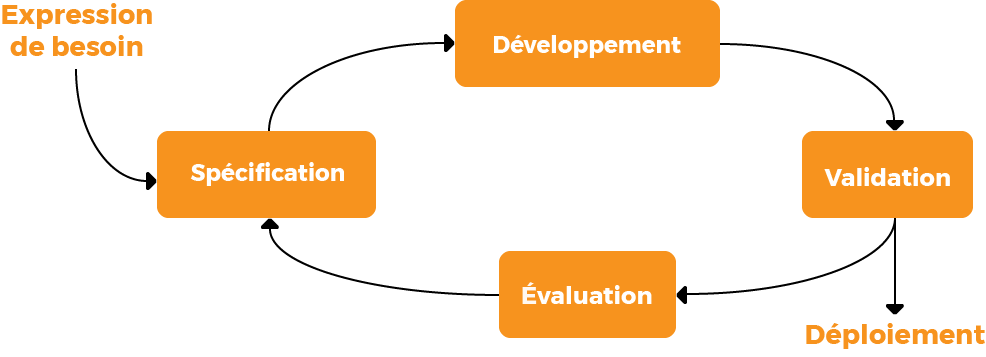
\includegraphics[width=0.8\textwidth]{contexte-generale/assets/cycleiteratif.png}
    \caption{Différentes étapes du cycle itératif}
    \label{fig:cycleiteratif}
\end{figure}

\subsubsection{Expression du besoin:}
La première réunion avec notre encadrant M. Mustapha AMEUR nous a permis de définir les différents besoins: 
\begin{itemize}
    \item Un outil d'analyse des sentiments à partir des tweets où l'utilisateur peut voir un score de positivité et de négativité de chaque tweet, en traçant graphiquement les variations selon le temps.  
\end{itemize}

Ça nous a permis aussi de définir les besoins non fonctionnels concernant notre système:
\begin{itemize}
    \item L’ergonomie : l’application offre une interface conviviale et facile à utiliser.
    \item Le code doit être clair et modulaire pour permettre des futures évolutions ou améliorations. Et d’être paramétrable le plus possible afin d’assurer une simplicité lors changements sans être obliger de modifier le code source.
\end{itemize}

\subsubsection{Spécification:}
Dans cette étape, nous avons choisi les différents outils et technologies qui vont nous aider à satisfaire les besoins définis dans la première étape: 
\begin{itemize}
    \item La conception et le développement d'une application desktop d'analyse des sentiments des tweets en temps réel en Python à l'aide de: Python-twitter, Vader, nltk, TextBlob, PyQt5. Comme on a décidé de former un modèle Naive Bayes basé sur notre propre "dataset". 
\end{itemize} 

\subsubsection{Développement:}
Dans cette étape, nous avons réalisé en concrèt ce qui a été définit en essayant de respecter un exemple d'un ensemble d'étapes de réalisation d'un projet en machine learning (Figure~\ref{fig:machinelearninglifecycle}):
\begin{figure}
    \centering
    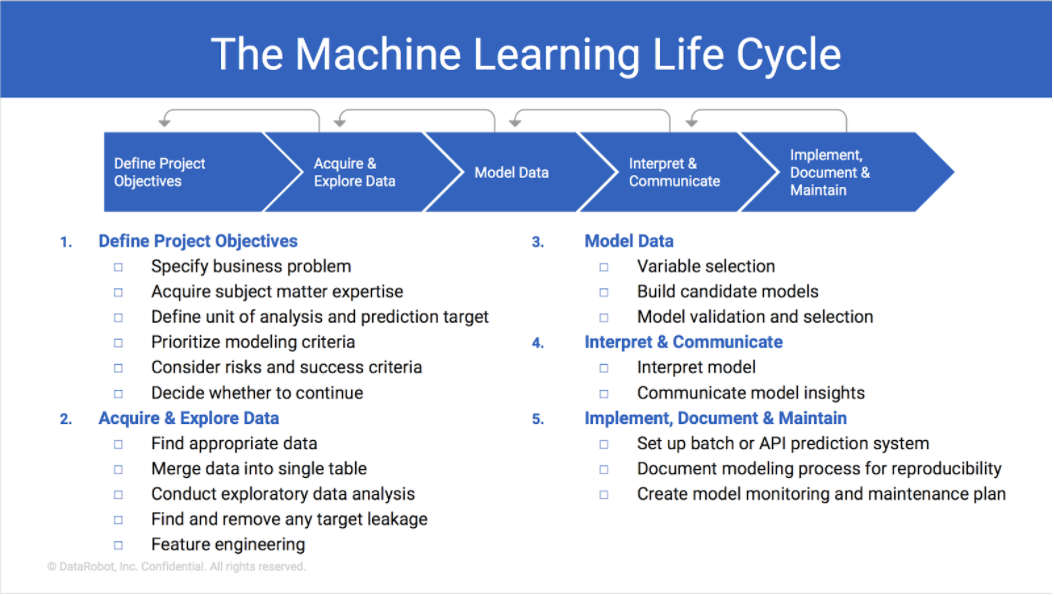
\includegraphics[width=0.9\textwidth]{contexte-generale/assets/machinelearning.png}
    \caption{Exemple d'étapes d'un projet en machine learning}
    \label{fig:machinelearninglifecycle}
\end{figure}

\subsubsection{Validation:}
Ensemble de test permettant d’assurer que le besoin initialement formulé est comblé.

\subsubsection{Évaluation:}
Cette étape nous a permis de faire le point sur les problèmes rencontrés lors des trois précédentes étapes, chose qui nous a aidé à trouver une solution pour accélerer le modèle entrainé (Naive Bayes) après quelques évaluations.

\subsubsection{Déploiement:}
les livrables validés sont déployés et prêts à être utilisé.

\section{Conclusion:}
Dans ce chapitre, nous avons présenter l'idée générale et le contexte de notre projet, comme on a détaillé la méthodologie du travail adaptée lors de la réalisation du projet.

\chapter{Étude théorique et conception}
\section{Étude préliminaire:}
Les méthodes existantes pour l'analyse des sentiments peuvent être regroupées en deux catégories principales: méthodes basées sur la connaissance (knowledge-based), ou sur l'apprentissage automatique (machine learning). \\
\subsection{Méthodes basées sur la connaissance: }
Dans les méthodes basées sur la connaissance, également appelé classification des sentiments basée sur le lexique, l'objectif est de
construire ou utiliser des lexiques de mots de sentiments existants avec des étiquettes de sentiments indiquées pour les mots
ou les phrases dans le texte. La classification du texte est définie par des règles; une fonction sur les mots, comme la somme des polarités des mots \cite{taboada2011lexicon}. Cette approche ne nécessite pas
toute formation (autre que la formation d'un lexique, si nécessaire). \\

Hu, Minqing et Bing Liu \cite{hu2004mining} ont construit un lexique, utilisant uniquement WordNet (base de données lexicale) et une liste d'adjectifs de semences étiquetés. Cette liste contient uniquement des adjectifs positifs (par exemple, grand, étonnant, agréable, cool) et des adjectifs négatifs (par exemple, mauvais, ennuyeux). Leur méthode récupère et étiquette automatiquement les synonymes (même polarité) et antonymes (polarité opposée). Ce processus permet à la liste de devenir un lexique. Un inconvénient de cette approche est qu'elle n'est applicable que dans les langues où WordNet est disponible. Dans tous les cas, la méthode basée sur les connaissances peut être difficile en raison du bruit dans les données textuelles, tandis que la création manuelle de règles pour combiner des informations sur les mots obtenus à partir des lexiques de sentiments prend du temps et des efforts.\\
\subsection{Méthodes basées sur l'apprentissage automatique: }
D'autre part, l'apprentissage automatique nécessite de former un modèle pour prédire la polarité du texte. Le modèle est formé avec des messages texte, étiquetés pour leur sentiment et représentés comme des vecteurs de fonctionnalités. Ce dernier nécessite classiquement un prétraitement de texte à l'aide d'outils de traitement de langage comme NLTK6. Le prétraitement du texte implique principalement la tokenisation, le stemming, le balisage et éventuellement l'analyse du texte. La sélection des caractéristiques appropriées à partir des données est cruciale et s'est révélée être un problème majeur et est toujours un objectif clé pour les chercheurs.\\

Des travaux antérieurs sur l'analyse des sentiments ont exploité des méthodes bien connues d'apprentissage automatique (machine learning) supervisé, telles que Naive Bayes \cite{martinez2006learning}, SVMs \cite{vinet2011missing, ho1995random,wahid2017prestasi}. Des travaux plus récents utilisent des modèles d'apprentissage profond (deep learning) \cite{goldberg2017neural}, en particulier les réseaux neuronaux récurrents (RNN) et le réseau neuronal convolutionnel (CNN). Cette thèse porte également sur les modèles d'apprentissage profond.
\begin{figure}[H]
    \centering
    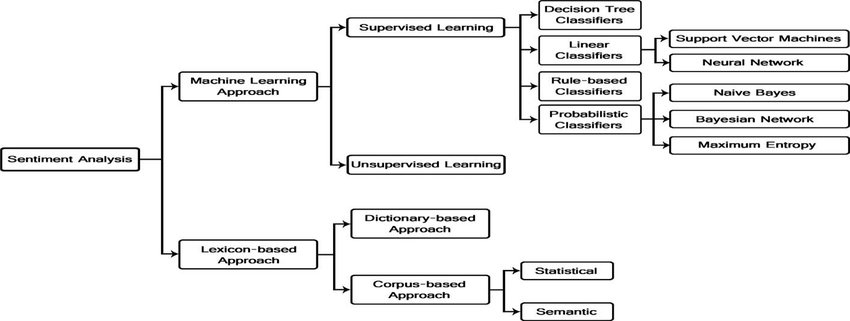
\includegraphics[width=\textwidth]{etude-theorique-conception/assets/sentiment-analysis-methods.jpg}
    \caption{Description des méthodes d'analyse des sentiments}
    \label{fig:my_label}
\end{figure}
\subsection{Limites des solutions existantes:}
Certaines limitations des solutions existantes de l'analyse des sentiments:
\begin{itemize}
    \item \textcolor{DispositionColor}{Pour les méthodes basées sur la connaissance:}
    \begin{itemize}
        \item Elles peuvent être difficile en raison du bruit dans les données textuelles, tandis que la création manuelle de règles pour combiner des informations sur les mots obtenus à partir des lexiques de sentiments prend du temps et des efforts.
        \item L'approche est qu'elle n'est applicable que dans les langues où le dictionnaire (La base de données lexicale) est disponible.
        \item Elles nécessitent de puissantes ressources linguistiques pour extraire des informations à partir des mots, chose qui n'existe pas toujours.
    \end{itemize}
    \item \textcolor{DispositionColor}{Pour les méthodes basées sur l'apprentissage automatique:}
    \begin{itemize}
        \item La sélection des caractéristiques appropriées à partir des données est cruciale et s'est révélée être un problème majeur et est toujours un objectif clé pour les chercheurs.
    \end{itemize}
\end{itemize}  
\section{NLP (Natural Language Processing):}
Le traitement du langage naturel est un sous-domaine de la linguistique, l'informatique, l'ingénierie de l'information et de l'intelligence artificielle concerné par les interactions entre les ordinateurs et les langues (naturelles) humaines, en particulier comment programmer des ordinateurs pour traiter et analyser de grandes quantités de données en langage naturel.\\

Les défis du traitement du langage naturel impliquent fréquemment la reconnaissance vocale, la compréhension du langage naturel et la génération du langage naturel.

\begin{figure}[H]
    \centering
    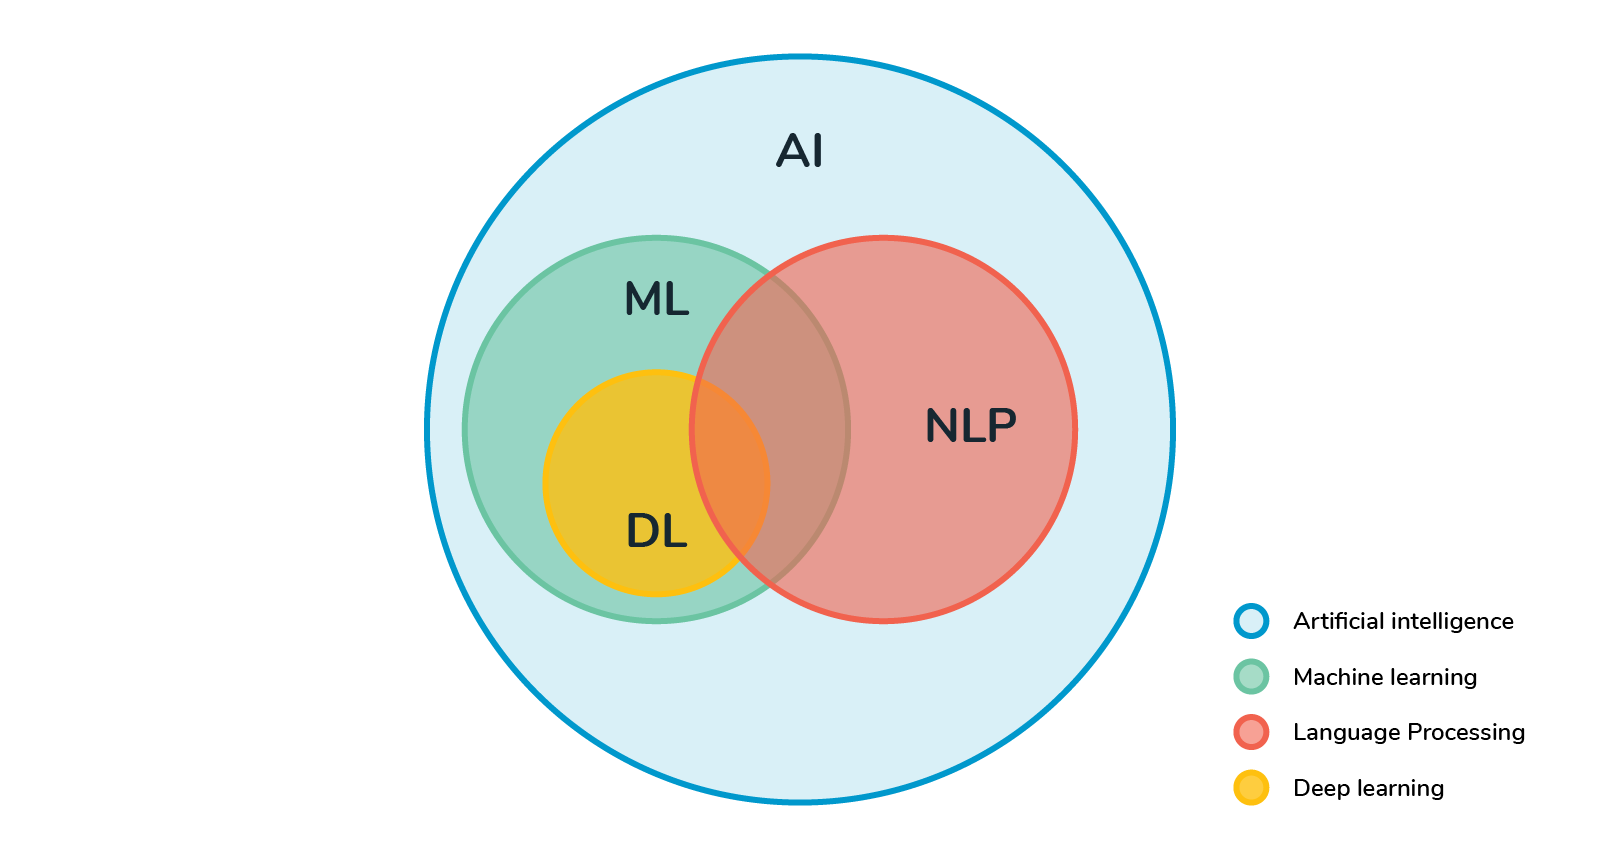
\includegraphics[width=\textwidth]{etude-theorique-conception/assets/nlp.png}
    \caption{NLP est une branche de l'intelligence artificielle}
    \label{fig:my_label}
\end{figure}

Ce qui suit est une liste des tâches les plus recherchées dans le traitement du langage naturel. Certaines de ces tâches ont des applications directes dans le monde réel, tandis que d'autres servent généralement de sous-tâches qui sont utilisées pour aider à résoudre des tâches plus importantes.\\

Bien que les tâches de traitement du langage naturel soient étroitement liées, elles sont fréquemment subdivisées en catégories pour plus de commodité:

\subsection{Syntaxe:}
\subsubsection{Induction grammaticale:}
La Génération d'une grammaire formelle qui décrit la syntaxe d'un langage. \\ \cite{klein2002natural}
\subsubsection{Lemmatisation:}
La tâche de supprimer uniquement les terminaisons flexionnelles et de renvoyer la forme de dictionnaire de base d'un mot qui est également connu sous le nom de lemme.
\subsubsection{Segmentation morphologique:}
La séparation des mots en morphèmes individuels et identifiez la classe des morphèmes. La difficulté de cette tâche dépend fortement de la complexité de la morphologie (c'est-à-dire la structure des mots) de la langue considérée.
\subsubsection{Segmentation des mots:}
La séparation d'un morceau de texte continu en mots séparés. Pour une langue comme l'anglais, c'est assez trivial, car les mots sont généralement séparés par des espaces. Cependant, certaines langues écrites ne marquent pas les limites des mots de cette manière, et dans ces langues, la segmentation du texte est une tâche difficile qui nécessite la connaissance du vocabulaire et de la morphologie des mots dans la langue.
\subsubsection{Catégorie grammaticale (Part-of-speech tagging):}
Cela implique d'identifier la catégorie grammaticale pour chaque mot.
\subsubsection{Analyse (Parsing):}
La détermination d'une arbre d'analyse (analyse grammaticale) d'une phrase donnée. La grammaire des langues naturelles est ambiguë et les phrases typiques ont de multiples analyses possibles. Peut-être de façon surprenante, pour une phrase typique, il peut y avoir des milliers d'analyses potentielles (dont la plupart sembleront complètement absurdes pour un humain).
\subsubsection{Rupture de phrase:}
Étant donné un morceau de texte, on trouve les limites de la phrase. Ces limites sont souvent marquées par des points ou d'autres signes de ponctuation, mais ces mêmes caractères peuvent servir à d'autres fins (par exemple, marquer des abréviations).
\subsubsection{"Stemming":}
Cela implique de couper les mots à leur forme racine.
\subsubsection{"Extraction terminologique":}
Le but de l'extraction terminologique est d'extraire automatiquement les termes pertinents d'un corpus donné.

\subsection{Sémantique:}
\subsubsection{Sémantique lexicale:}
La signification informatique des mots individuels dans leur contexte.
\subsubsection{Sémantique distributionnelle:}
L'apprentissage des représentations sémantiques à partir des données.
\subsubsection{Reconnaissance des entités nommées:}
Il s'agit de déterminer les parties d'un texte qui peuvent être identifiées et classées en groupes prédéfinis. Par exemple les noms de personnes et les noms de lieux.
\subsubsection{Désambiguïsation du sens des mots:}
Beaucoup de mots ont plus d'un sens; nous devons sélectionner le sens qui est le plus convenable au contexte. Pour ce problème, on reçoit généralement une liste de mots et de sens de mots associés, par exemple à partir d'un dictionnaire ou d'une ressource en ligne telle que WordNet.
\subsubsection{Extraction de relations:}
Étant donné un morceau de texte, on identifie les relations entre les entités nommées.
\subsubsection{Génération du langage naturel:}
Il s'agit d'utiliser des bases de données pour dériver des intentions sémantiques et les convertir en langage humain.
\subsection{Discours:}
\subsubsection{Synthèse automatique:}
La production d'un résumé lisible d'un morceau de texte.
\subsubsection{Résolution de coréférence:}
Étant donné une phrase ou un morceau de texte, on détermine quels mots (mentions) font référence aux mêmes objets (entités).
\subsection{Parole:}
\subsubsection{Reconnaissance de la parole:}
À partir d'un extrait sonore d'une ou de plusieurs personnes parlant, on détermine la représentation textuelle du discours.
\subsubsection{Segmentation de la parole:}
Étant donné un extrait sonore d'une ou de plusieurs personnes parlant, on le sépare en mots. Une sous-tâche de reconnaissance vocale et généralement regroupée avec elle.
\subsubsection{Synthèse de la parole à partir du texte (Text-to-speech)}
Étant donné un texte, on transforme ses unités et on produit une représentation parlée. La synthèse vocale peut être utilisée pour aider les gens avec une basse vision. \cite{yi2011assistive}


\begin{figure}[H]
    \centering
    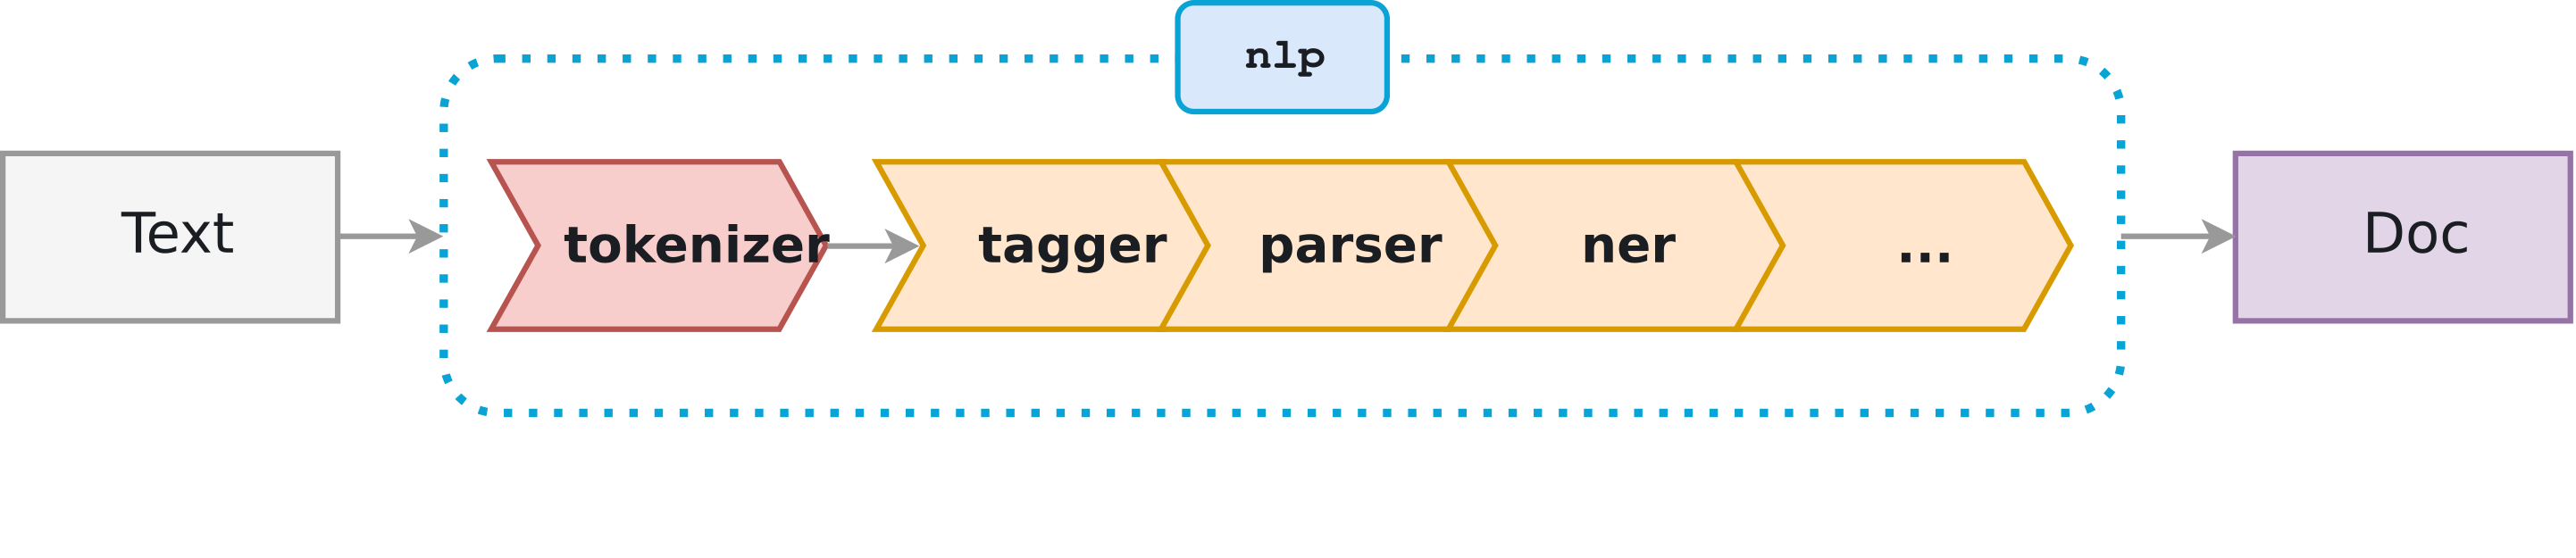
\includegraphics[width=\textwidth]{etude-theorique-conception/assets/nlp1.png}
    \caption{Processus NLP}
    \label{fig:my_label}
\end{figure}

\section{Algorithme Naive Bayes:}
L'algorithme Naive Bayes est un algorithme de classification probabiliste simple qui s'appuie sur le théorème de Bayes. Naive Bayes a des hypothèses d'indépendance fortes (naïves) entre les caractéristiques. En termes simples, un classificateur Naive Bayes suppose que la présence d'une caractéristique particulière dans une classe n'est pas liée à la présence de toute autre caractéristique. Par exemple, un ballon peut être considéré comme un ballon de football s'il est dur, rond et d'environ sept pouces de diamètre. Même si ces caractéristiques dépendent les unes des autres ou de l'existence des autres caractéristiques, Bayes naïf pense que toutes ces propriétés contribuent indépendamment à la probabilité que ce ballon soit un ballon de football, c'est pourquoi il est connu comme naïf. \\

Les modèles Naive Bayes sont faciles à construire. Ils sont également très utiles pour de très grands ensembles de données. Bien que les modèles Bayes naïfs soient simples, ils sont connus pour surpasser même les modèles de classification les plus sophistiqués. Parce qu'ils nécessitent également un temps de formation relativement court, ils constituent une bonne alternative pour une utilisation dans les problèmes de classification. \\

Résuméement, Bayes naïf est un modèle de probabilité conditionnel: étant donné une instance de problème à classer, représentée par un vecteur $x=x_{1},...,x_{n}$  représentant n fonctionnalités (variables indépendantes), il assigne à cette instance des probabilités ${p(C_{k}| x_{1},...,x_{n})}$ pour chaque $K$ résultats ou classes possibles ou classes $C_{k}$. \cite{murty2011pattern} \\

Le problème avec la formulation ci-dessus est que si le nombre d'entités n est grand ou si une entité peut prendre un grand nombre de valeurs, alors baser un tel modèle sur des tables de probabilités est irréalisable. Nous reformulons donc le modèle pour le rendre plus maniable. En utilisant le théorème de Bayes, la probabilité conditionnelle peut être décomposée comme:
\begin{equation}
    P(C_{k} | X)=\frac{P(X | C_{k}) P(C_{k})}{P(X)}
\end{equation}

En pratique, il n'y a d'intérêt que pour le numérateur de cette fraction, car le dénominateur ne dépend pas de $C$ et les valeurs des traits $x_ {i}$ sont données, de sorte que le dénominateur est effectivement constant. Le numérateur est équivalent au modèle de probabilité conjoint ${p(C_{k},x_{1},...,x_{n})}$ qui peut être réécrite comme suit, en utilisant la règle de chaîne de la définition de la probabilité conditionnelle:
\begin{equation}
    \begin{aligned}
    p\left(C_{k}, x_{1}, \ldots, x_{n}\right) &=p\left(x_{1}, \ldots, x_{n}, C_{k}\right) \\
    &=p\left(x_{1} | x_{2}, \ldots, x_{n}, C_{k}\right) p\left(x_{2}, \ldots, x_{n}, C_{k}\right) \\
    &=p\left(x_{1} | x_{2}, \ldots, x_{n}, C_{k}\right) p\left(x_{2} | x_{3}, \ldots, x_{n}, C_{k}\right) p\left(x_{3}, \ldots, x_{n}, C_{k}\right) \\
    &=\cdots \\
    &=p\left(x_{1} | x_{2}, \ldots, x_{n}, C_{k}\right) p\left(x_{2} | x_{3}, \ldots, x_{n}, C_{k}\right) \ldots p\left(x_{n-1} | x_{n}, C_{k}\right) p\left(x_{n} | C_{k}\right) p\left(C_{k}\right)
    \end{aligned}
\end{equation}

Maintenant, les hypothèses d'indépendance conditionnelle "naïve" entrent en jeu: supposons que toutes les fonctionnalités de $x$ sont mutuellement indépendantes, conditionnelles à la catégorie $C_{k}$, dans cette hypothèse, $
    p\left(x_{i} | x_{i+1}, \ldots, x_{n}, C_{k}\right)=p\left(x_{i} | C_{k}\right)
    $ \\

Ainsi, le modèle commun peut être exprimé comme: 
\begin{equation}
    \begin{aligned}
    p\left(C_{k} | x_{1}, \ldots, x_{n}\right) & \propto p\left(C_{k}, x_{1}, \ldots, x_{n}\right) \\
    &=p\left(C_{k}\right) p\left(x_{1} | C_{k}\right) p\left(x_{2} | C_{k}\right) p\left(x_{3} | C_{k}\right) \cdots \\
    &=p\left(C_{k}\right) \prod_{i=1}^{n} p\left(x_{i} | C_{k}\right)
    \end{aligned}
\end{equation}
où $\propto$ dénote la proportionnalité. \\

Cela signifie que sous les hypothèses d'indépendance ci-dessus, la distribution conditionnelle sur la variable de classe $C$ est: \\
\begin{center}
    $p\left(C_{k} | x_{1}, \ldots, x_{n}\right)=\frac{1}{Z} p\left(C_{k}\right) \prod_{i=1}^{n} p\left(x_{i} | C_{k}\right)$
\end{center}
où $Z=p(\mathbf{x})=\sum_{k} p\left(C_{k}\right) p\left(\mathbf{x} | C_{k}\right)$ $x_{1}, \ldots, x_{n}$ c'est-à-dire une constante si les valeurs des variables d'entité sont connues.
\paragraph{Construire un classificateur à partir du modèle de probabilité:}
Jusqu'à présent, la discussion a dérivé le modèle d'entité indépendant, c'est-à-dire le modèle de probabilité naïf de Bayes. Le classificateur naïf de Bayes combine ce modèle avec une règle de décision. Une règle courante consiste à choisir l'hypothèse la plus probable; il s'agit de la règle de décision maximale a posteriori ou MAP(maximum a posteriori). Le classificateur Bayes, est la fonction qui attribue une étiquette de classe ${\displaystyle {\hat{y}} = C_ {k}}$ pour certains $k$ comme suit: \\
\begin{center}
    $\hat{y}=\underset{k \in\{1, \ldots, K\}}{\operatorname{argmax}} p\left(C_{k}\right) \prod_{i=1}^{n} p\left(x_{i} | C_{k}\right)$  
\end{center}


\section{Vader:}
Vader (Valence Aware Dictionary and sentiment Reasoner) est un lexique et un outil d'analyse des sentiments basé sur des règles, qui est spécifiquement adapté aux sentiments exprimés dans les médias sociaux. Vader utilise une combinaison d'un lexique de sentiments qui est une liste de caractéristiques lexicales généralement étiquetées selon leur orientation sémantique comme positives ou négatives.\\

Vader s'est avéré très efficace dans le traitement de textes de médias sociaux, de critiques de films et de produits. Cela est dû au fait que Vader ne parle pas seulement du score de positivité et de négativité, mais nous indique également à quel point un sentiment est positif ou négatif (compound).\cite{hutto2014Vader}\\


\subsection{Quantifier l'émotion d'un mot:}
L'analyse des sentiments Vader s'appuie principalement sur un dictionnaire qui mappe les caractéristiques lexicales aux intensités émotionnelles appelées scores des sentiments. Le score de sentiment d'un texte peut être obtenu en résumant l'intensité de chaque mot dans le texte. Et par caractéristiques lexicales, on veut dire tout ce que nous utilisons pour la communication textuelle (mots, "emojis" au cas de l'analyse des tweets par exemple, acronymes...) \\

L'intensité d'émotion ou le score de sentiment est mesuré sur une échelle de -4 à +4, où -4 est le plus négatif et +4 est le plus positif. Le point médian 0 représente un sentiment neutre.\\

Vader construit son dictionnaire en utilisant les évaluateurs humains d'Amazon Mechanical Turk, et pour contrer la subjectivité des évaluateurs (notions différentes de ce qui est ositif ou negatif), les créateurs de Vader ont utilisé non seulement un, mais un certain nombre d'évaluateurs humains et ont fait la moyenne de leurs notes pour chaque mot. Cela repose sur le concept de la sagesse de la foule (the wisdom of the crowd).
\subsection{Quantifier l'émotion d'une phrase:}
L'analyse de sentiment Vader renvoie un score de sentiment compris entre -1 et 1, du plus négatif au plus positif en sommant les scores de sentiment de chaque mot de la phrase existant dans le dictionnaire Vader avant de normaliser cette somme pour le mapper à une valeur comprise entre -1 et 1. La normalisation utilisée par \cite{hutto2014Vader}: \\ 
\begin{center}
    $\frac{x}{\sqrt{x^{2}+\alpha}}$ 
\end{center}

$x$ est la somme des scores de sentiment des mots constitutifs de la phrase et $\alpha$ est un paramètre de normalisation que nous fixons à 15. La normalisation est représentée graphiquement ci-dessous.
\begin{figure}[H]
    \centering
    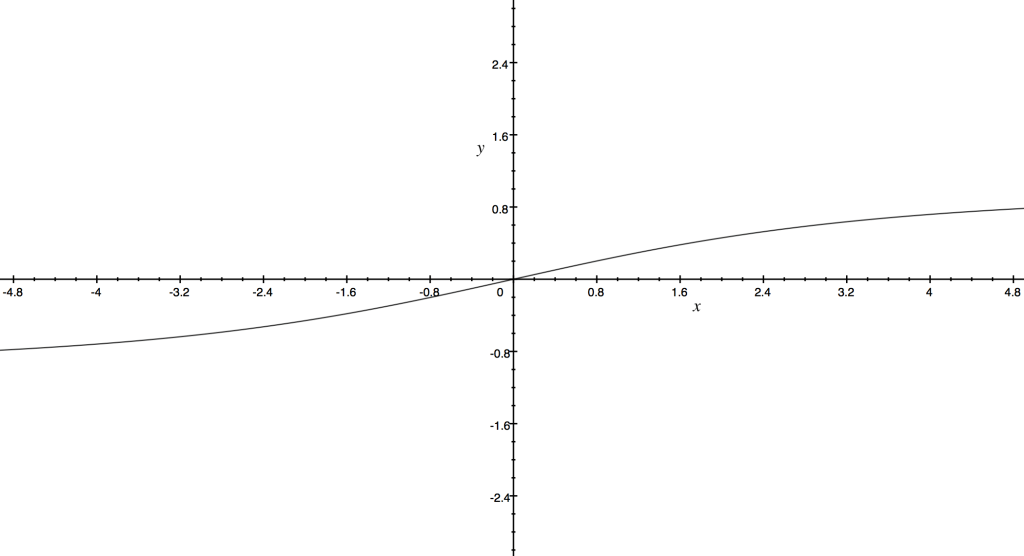
\includegraphics[width=0.6\textwidth]{etude-theorique-conception/assets/vader-normalization.png}
    \caption{Normalisation de Vader}
    \label{fig:my_label}
\end{figure}
Nous voyons ici que lorsque $x$ grandit, il devient de plus en plus proche de -1 ou 1. Pour un effet similaire, s'il y a beaucoup de mots dans le document auquel vous appliquez l'analyse des sentiments Vader, on obtient un score proche de -1 ou 1. Ainsi,l'analyse des sentiments Vader fonctionne mieux sur les documents courts, comme les tweets et les phrases, pas sur les gros documents.

\section{Conception du système:}
Dans cette étape, nous abordons la partie conception du projet, dans laquelle, nous
détaillons les différents éléments de conception, en commançant d'abord par spécificier les besoins fonctionnels de notre système, établir une architecture générale puis une modélisation statique du système à travers un diagramme de classes.
\subsection{Spécification des besoins fonctionnels:}
La spécification de ces besoins va nous permettre d’avoir une meilleure approche des utilisateurs, des fonctionnalités et de la relation entre les deux. Elle sera alors sous forme d'un diagramme de cas d’utilisation où on va procéder par l'identification des acteurs agissant sur notre système et les différentes cas d'utilisation: \\
\begin{figure}[H]
    \centering
    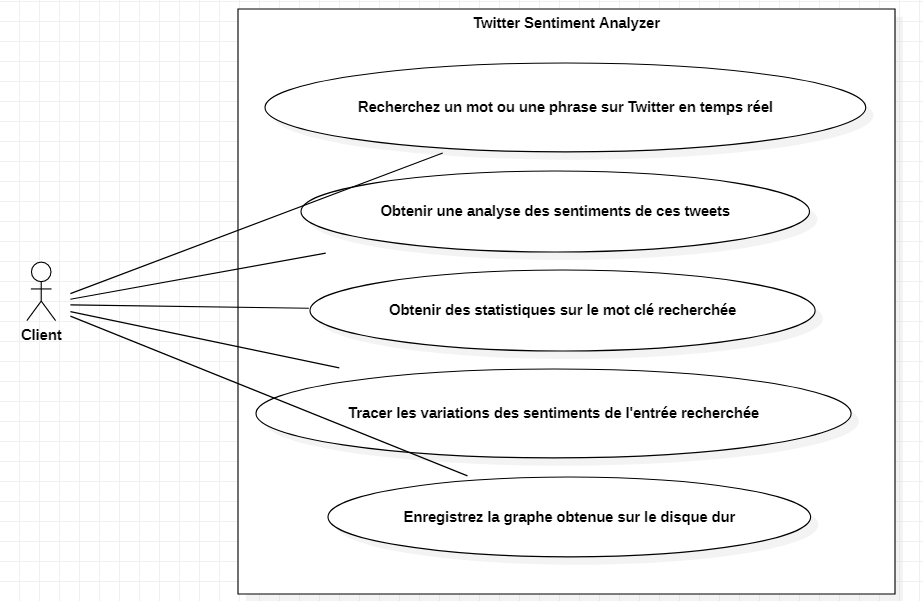
\includegraphics[width=\textwidth]{etude-theorique-conception/assets/useCase.png}
    \caption{Diagramme de cas d'utilisation}
    \label{fig:my_label}
\end{figure}
\subsection{Architecture générale de la solution:}
Pour réaliser notre système, on a choisi à suivre une architecture adapté à la nature de notre projet que nous représentons dans ce diagramme:
\begin{figure}[H]
    \centering
    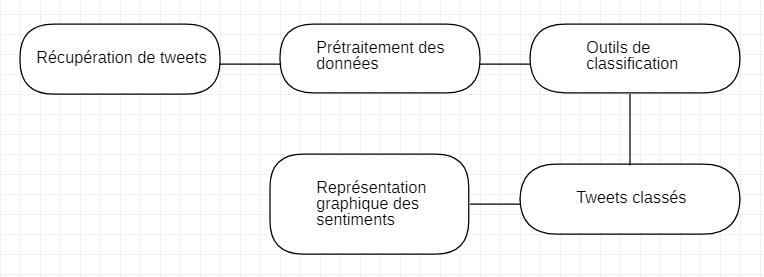
\includegraphics[width=\textwidth]{etude-theorique-conception/assets/architecture.png}
    \caption{Architecture du système}
    \label{fig:my_label}
\end{figure}
Comme on remarque dans le diagramme ci-dessus, on peut diviser le fonctionnement de notre application en cinque grandes parties:
\begin{itemize}
    \item \textcolor{DispositionColor}{Récupération de tweets:} La recherche et l'extraction des tweets contenant le mot clé entré par l'utilisateurs.
    \item \textcolor{DispositionColor}{Prétraitement des données:} Cette partie consiste à appliquer les différentes tâches et techniques de "NLP" pour traiter les tweets récupérés.
    \item \textcolor{DispositionColor}{Outils de classification:} Définir les méthodes suivies pour l'analyse de sentiments et la classification des tweets. 
    \item \textcolor{DispositionColor}{Tweets classés:} Classer ces tweets par des labels (positif ou négatif par exemple) et donner une évaluation générale sur l'ensemble de tweets récupérés.  
    \item \textcolor{DispositionColor}{Représentation graphique des sentiments:} Représentation graphique des sentiments de tweets selon les méthodes d'analyse choisie.
\end{itemize}
\subsection{Diagramme de classes:}
Le diagramme de classes est une modélisation statique du système en termes de classes et
de relations entre ces classes. Son intérêt réside dans la modélisation des entités du
système d'information.\\

Vu la nature de notre projet, nous avons décidé de créer deux entités illustrées dans le diagramme suivant:
\begin{figure}[H]
    \centering
    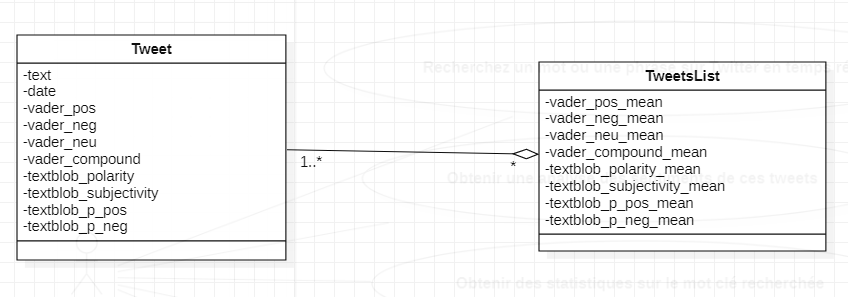
\includegraphics[width=\textwidth]{etude-theorique-conception/assets/classDiagram.png}
    \caption{Diagramme de classes}
    \label{fig:my_label}
\end{figure}
\begin{itemize}
    \item \textcolor{DispositionColor}{Tweet:} On utilise cette classe pour stocker les différentes informations liées à chaque tweet récupérés.
    \item \textcolor{DispositionColor}{TweetsList:} On utilise cette classe pour stocker les informations liées à l'ensemble de tweets récupérés.
\end{itemize}
\section{Conclusion:}
Dans ce chapitre, nous avons effectué une étude théorique où on a exploré les différents concepts utilisé pour la réalisation du projet, comme on a abordé le côté conceptuel du projet. 




\chapter{Les choix techniques}

\section{Solution détaillée:}
Notre solution consiste à concevoir et développer une application d'analyse des sentiments des tweets en temps réel en utilisant les outils et les librairies suivantes:
\begin{itemize}
    \item Chercher les tweets contenant le mot clé entré, en utilisant \bb{python-twitter}, la librairie qui fournit une interface Python pure pour utiliser l'API Twitter.
    \item Analyser ces tweets à travers des models fournis par \bb{TextBlob}, \bb{Vader}, \bb{nltk}, et par un modèle Naive Bayes formé par nous-même, pour obtenir des statistiques sur le mot clé entré.
    \item Tracer les changements des sentiments de ces tweets.
    \item Donner la possibilité de sauvegarder les graphes tracées, ainsi que les tweets et ses analyses, sur le disque dur sous plusieurs formats (PNG, JPEG...).
\end{itemize}

L'interaction avec l'utilisateur se fait via une interface graphique réalisée à l'aide de \bb{PyQt5} (l'ensemble de liaisons Python pour Qt), où s'affichent les tweets, les différentes statistiques ainsi que les graphes tracées.

\section{Environnement logiciel:}
Nous avons intérêt à mettre en place une architecture rigoureuse, de manière à garantir la
maintenabilité, l'évolutivité et l'exploitabilité de notre application.

\subsection{Python:}
La nature de notre projet (Analyse de sentiments) nous a poussé à choisir Python pour le développement de notre application surtout qu'il est le langage le plus populaire pour les projets d'intelligence artificielle, "machine learning", et le "deep learning": \cite{python}

Python nous offre alors:
\subsubsection{Un grand écosystème de bibliothèques:}
Un grand choix de bibliothèques est l'une des principales raisons pour lesquelles Python est le langage de programmation le plus populaire utilisé pour l'intelligence artificielle et le "machine learning", surtout que ce dernier nécessite un traitement continu des données, et les bibliothèques Python nous permettent d'accéder, de gérer et de transformer les données.

On mentionne comme exemple: Scikit-learn, Pandas, TensorFlow, Matplotlib, NLTK, etc.

\subsubsection{Flexibilité:}
Il offre l'option pour choisir entre utiliser POO ou la méthode fonctionnelle, et il n'est pas non plus nécessaire de recompiler le code source, les développeurs peuvent implémenter toutes les modifications et voir rapidement les résultats, comme ils peuvent combiner Python et d'autres langages pour atteindre leurs objectifs.

\subsubsection{Lisibilité:}
Python est très facile à lire pour que chaque développeur Python puisse comprendre le code de ses pairs et le modifier, le copier ou le partager. Il n'y a pas de confusion, d'erreurs ou de paradigmes conflictuels, ce qui conduit à un échange plus efficace d'algorithmes, d'idées et d'outils.

\subsection{Jupyter Notebook:}
Le "notebook" étend l'approche basée sur la console à l'informatique interactive dans une nouvelle direction qualitative, en fournissant une application Web adaptée à la capture de l'ensemble du processus de calcul: développement, documentation et exécution de code, ainsi que communication des résultats. Le bloc-notes Jupyter combine deux composants:
\begin{itemize}
    \item \bb{Une application Web:} Un outil basé sur un navigateur pour la création interactive de documents qui combinent du texte explicatif, des mathématiques, des calculs et leur output media.
    \item \bb{Documents "notebook":} Une représentation de tout le contenu visible dans l'application Web, y compris les entrées et sorties des calculs, le texte explicatif, les mathématiques, les images et les représentations media des objets.
\end{itemize}

\subsection{Google Colab:}
Google a fourni un service cloud gratuit basé sur les "Jupyter Notebooks" qui prend en charge le GPU gratuit. Google Colab nous permet de développer des applications de "deep learning" à l'aide de bibliothèques populaires telles que PyTorch, TensorFlow, Keras et OpenCV.

On peut créer des "notebooks" dans Colab, les télécharger, les stocker, les partager, monter Google Drive et utiliser tout ce qu'on y a stocké, importer la plupart de nos répertoires préférés, télécharger des "notebooks" directement depuis GitHub, téléchargez des fichiers Kaggle, et plein d'autre fonctionnalités~\cite{googlecolab}.

\section{Conclusion:}
Dans ce chpitre, nous avons présenté notre solution envisagée ainsi que l'environnement logiciel dans laquelle nous avons réalisé notre projet.





\chapter{Réalisation}
\section{Introduction}
Pour faciliter le travail, nous avons utilisé Pyqt5 pour l'implémentation d'une GUI, des modèles pré-formés pour nous aider à obtenir des résultats rapides, et nous avons choisi de former nous-mêmes un modèle "Naive Bayes" sur un ensemble de tweets de 2009 Annexe~\ref{naivebayesimplementation}. L'ensemble de données est composé de plus de 1,6 millions de tweets.
\section{Notre implémenation de Naive Bayes:} 
Pour former notre modèle Bayes naïf, nous importons les données brutes de notre base de données CSV comme suit:\\
\begin{table}[h!]
\centering
    \begin{tabular}{|c|c|} 
    \hline
    score & texte \\ [0.5ex] 
    \hline\hline
    0 & @switchfoot http://twitpic.com/2y1zl - Awww, t... \\ 
    \hline
    0 & is upset that he can't update his Facebook by... \\
    \hline
    0 & @Kenichan I dived many times for the ball. Man... \\
    \hline
    0 & my whole body feels itchy and like its on fire \\
    \hline
    0 & @nationwideclass no, it's not behaving at all.... \\ [0.5ex] 
    \hline
   \end{tabular}
   \caption{Données brutes pour former notre modèle}
   \label{table:1}
\end{table}
Ces tweets bruts doivent être prétraités dans d'autres pour que les Bayes naïfs les utilisent comme un ensemble d'entraînement. Nous ouvrons les tweets chez les pandas pour faciliter la manipulation. Nous choisissons uniquement ce qui nous intéresse dans les colonnes: le texte et la partition.\\

L'ensemble de données est ordonné en deux catégories, positives et négatives. Nous avons donc dû mélanger l'ensemble de données pour créer une distribution aléatoire des entrées et obtenir un ensemble équilibré pour la formation et les tests.\\

Le prétraitement des tweets devait se faire en plusieurs étapes:
\begin{itemize}
    \item Convertir tous les mots en minuscules pour assurer l'homogénéité des tweets et du dictionnaire;
    \item Supprimer les URL et les remplacer par le mot clé "URL" pour préserver l'intégrité des tweets;
    \item Supprimer les marques \@ et les remplacer par le mot-clé "AT\_USER";
    \item Retirez le signe du hashtag;
    \item Tokenize les tweets pour supprimer les caractères répétés puis les diviser en mots;
    \item Tout d'abord, nous avons dû supprimer les mots inutiles basés sur la bibliothèque "stopwords" de NLTK;
\end{itemize}

Après le prétraitement de tous les tweets, nous avons divisé l'ensemble de données en un ensemble d'apprentissage de 95\% de tous les tweets et de 5\% pour le test. \\

Sur la base des tweets traités, nous construisons le dictionnaire de vocabulaire, qui sera utilisé pour faire correspondre les mots avec leur index correspondant, pour permettre au modèle de s'entraîner sur ces index.\\

La formation sur les serveurs Tensor Processing Unit sur Google Colab se bloquait si nous utilisions plus de 100 000 tweets. Nous avons donc opté pour la formation du modèle sur 5000 tweets de base afin de permettre au serveur de gérer le mot et de ne pas prendre plus de 6 heures.

Nous avons obtenu un résultat respectable pour les paramètres par défaut avec une précision de 84\%.\\

Nous enregistrons les poids et les paramètres du modèle à l'aide de cornichons (pickles) et du vocabulaire dans un fichier CSV utilisé pour la prochaine utilisation.
\section{Librairies et APIs utilisés:}
\subsection{Python-Twitter:}
C'est une bibliothèque qui fournit une interface Python pure pour l'API Twitter. Twitter met en disposition un service qui permet aux gens de se connecter via le Web, la messagerie instantanée et les SMS, Twitter expose alors une API Web et cette bibliothèque a pour but de la rendre encore plus facile à utiliser pour les programmeurs Python.\cite{py-twitter}
\subsubsection{Twitter API:}
À un niveau élevé, les API sont la façon dont les programmes informatiques se «parlent» les uns aux autres pour pouvoir demander et fournir des informations. Pour ce faire, une application logicielle peut appeler ce que l'on appelle un point de terminaison:
une adresse qui correspond à un type spécifique d'informations fournis (les points de terminaison (endpoints) sont généralement uniques comme les numéros de téléphone).
Twitter permet d'accéder à certaines parties de l'API pour permettre aux utilisateurs de créer un logiciel qui s'intègre à Twitter.\cite{twitterAPI} \\

Les données Twitter sont uniques par rapport aux données partagées par la plupart des autres plateformes sociales car elles reflètent les informations que les utilisateurs choisissent de partager publiquement, et cet API nous donne l'accès à ces données.
L'API prend également en charge les API qui permettent aux utilisateurs de gérer leurs propres informations Twitter non publiques (par exemple, les messages directs) et de fournir ces informations aux développeurs qu'ils ont autorisés à le faire.
\paragraph{Accéder aux données Twitter:} 
Par défaut, les applications ne peuvent accéder qu'aux informations publiques sur Twitter. Certains points de terminaison (endpoints), tels que ceux chargés d'envoyer ou de recevoir des messages directs, nécessitent des autorisations supplémentaires de la part de l'utilisateur avant de pouvoir accéder à ses informations, et ces autorisations ne sont pas accordées par défaut. \\

L'API Twitter inclut un large éventail de points de terminaison, qui se répartissent en cinq groupes principaux:
\begin{itemize}
    \item \textcolor{DispositionColor}{Comptes et utilisateurs:} L'API permet aux développeurs de gérer (par programme) le profil et les paramètres d'un compte, de désactiver ou de bloquer les utilisateurs, de gérer les utilisateurs et les abonnés, de demander des informations sur l'activité d'un compte autorisé, et d'autres fonctionnalités.
    \item \textcolor{DispositionColor}{Tweets et réponses:} L'API met les Tweets et les réponses publiques à la disposition des développeurs et permet à ces derniers de publier des Tweets. Les développeurs peuvent accéder aux Tweets en recherchant des mots clés spécifiques ou en demandant un échantillon de Tweets à des comptes spécifiques.
    \item \textcolor{DispositionColor}{Messages directs:} Les points de terminaison de message direct permettent d'accéder aux conversations DM des utilisateurs qui ont explicitement accordé l'autorisation à une application spécifique, ils fournissent un accès limité aux développeurs pour créer des expériences personnalisées sur Twitter. Par exemple pour les comptes qu'elles possèdent ou gèrent, les entreprises peuvent créer ces expériences conversationnelles alimentées par des humains ou des "chatbots" pour communiquer directement avec les clients.
    \item \textcolor{DispositionColor}{Les publicités:} Twitter met à disposition une suite d'API pour permettre aux développeurs d'aider les entreprises à créer et gérer automatiquement des campagnes publicitaires sur Twitter. Les développeurs peuvent utiliser des Tweets publics pour identifier les sujets et les intérêts, et fournir aux entreprises des outils pour lancer des campagnes publicitaires pour atteindre les divers publics sur Twitter.
    \item \textcolor{DispositionColor}{Outils de l'éditeur et SDK:} L'API fournit aussi des outils aux développeurs et éditeurs de logiciels pour intégrer des boutons de partage et d'autres contenus Twitter sur des pages Web. Ces outils permettent aux développeurs d'intégrer des conversations publiques en direct de Twitter dans leurs plateformes et facilitent le partage d'informations et d'articles de leurs sites avec les utilisateurs.
\end{itemize}
\subsection{NLTK:}
NLTK (Natural Language Toolkit) est une plate-forme leader pour la construction de programmes Python pour travailler avec des données de langage humain. Il fournit des interfaces faciles à utiliser à plus de 50 corpus et ressources lexicales telles que WordNet, ainsi qu'une suite de bibliothèques de traitement de texte pour la classification, la tokenisation, le stemming, le balisage, l'analyse et le raisonnement sémantique. En autre mot, NLTK aide la machine à analyser, prétraiter et comprendre le texte écrit.\cite{bird2009natural}
\subsubsection{Tokenization:}
"Tokenization" est la première étape de l'analyse de texte. Le processus de décomposition d'un paragraphe de texte en morceaux plus petits tels que des mots ou des phrases est appelé "Tokenization". Le jeton (token) est une entité unique qui constitue des blocs de construction pour une phrase ou un paragraphe.
\subsubsection{Distribution de fréquence:}
NLTK nous permet aussi à calculer la fréquence correspondante à chaque mot donné.
\begin{figure}[H]
    \centering
    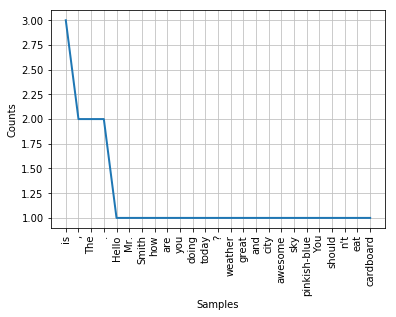
\includegraphics[width=0.8\textwidth]{realisation/assets/nltk-freq.png}
    \caption{Exemple d'une représentation de la distribution de fréquence}
    \label{fig:my_label}
\end{figure}
\subsubsection{Mots vides (Stopwords):}
Pour supprimer les mots vides dans NLTK, on doit créer une liste de mots vides et filtrer la liste de jetons à partir de ces mots.
\subsubsection{Normalisation du lexique:}
La normalisation du lexique considère un autre type de bruit dans le texte. Par exemple, "connexion", "connecté", "connectant" se réduit à un mot commun "se connecter". Il réduit les formes dérivées d'un mot à un mot racine commun.
\paragraph{Stemming:}
Le "Stemming" est un processus de normalisation linguistique, qui réduit les mots à leur mot racine ou coupe les affixes de dérivation.
\paragraph{Lemmatisation:}
La lemmatisation réduit les mots à leur mot de base.
\subsubsection{Balisage par catégorie grammaticale (POS tagging):}
L'identification du groupe grammatical d'un mot donné.
\begin{figure}[H]
    \centering
    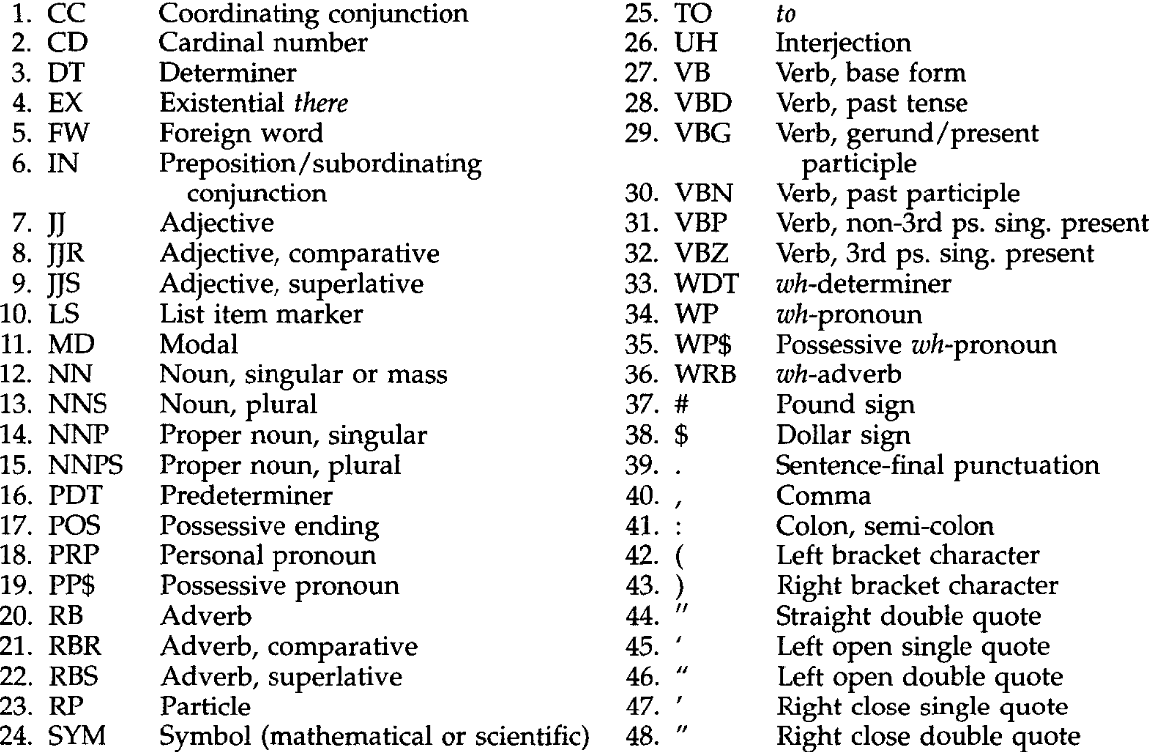
\includegraphics[width=\textwidth]{realisation/assets/nltk-pos.png}
    \caption{Différents "POS tags" pour la langue anglaise}
    \label{fig:my_label}
\end{figure}
\subsection{TextBlob:}
TextBlob est une bibliothèque Python pour le traitement de données textuelles. Il fournit une API simple pour plonger dans des tâches courantes de traitement du langage naturel (NLP) \cite{loria2018textblob}, il nous permet d'analyser les sentiments d'un texte et classer le résultat en deux catégories:
\begin{itemize}
    \item \textcolor{DispositionColor}{Polarité:} est une valeur flottante dans la plage [-1,0 à 1,0] où 0 indique neutre, +1 indique un sentiment très positif et -1 représente un sentiment très négatif.
    \item \textcolor{DispositionColor}{Subjectivité:} est une valeur flottante dans la plage [0,0 à 1,0] où 0 est très objectif et 1 est très subjectif. La phrase subjective exprime certains sentiments personnels, vues, croyances, opinions, allégations, désirs, croyances, soupçons et spéculations alors que les phrases objectives sont factuelles.
\end{itemize}
TextBlob est en fait construit sur NLTK et Pattern (un autre module de traitement de données textuelles), il fournit une interface facile à utiliser à la bibliothèque NLTK, et nous permet donc d'utiliser une variété de fonctionnalités telles que le balisage par catégorie grammaticale (POS tagging), "Tokenization", "Stemming", Lemmatisation et bien d'autres:
\subsubsection{Convertir le texte au singulier et au pluriel:}
Quand on passe le texte qu'on veut analyser comme paramètre à la classe "TextBlob", TextBlob nous permet de convertir l'objet retourné au singulier ou au pluriel à l'aide de deux méthode: "singularize()" et "pluralize()".
\subsubsection{Extraction de phrases nominales:}
L'extraction de phrases nominales, comme son nom l'indique, fait référence à l'extraction de phrases débutant avec des noms. Pour le faire on doit simplement utiliser les attributs "noun\_phrase" sur l'objet TextBlob.
\subsubsection{Correction d'orthographe:}
La correction d'orthographe est l'une des fonctionnalités uniques de TextBlob. Avec la méthode "correct()" de l'objet TextBlob, on peut corriger toutes les fautes d'orthographe dans votre texte.
\subsubsection{Traduction de la langue:}
L'une des capacités les plus puissantes de TextBlob est de traduire d'une langue à une autre. Sur le backend, le traducteur de langue TextBlob utilise l'API Google Translate. Il suffit de passer le texte à l'objet TextBlob puis d'appeler la méthode "translate" sur l'objet. Le code de langue souhaitée comme résultat est transmis en tant que paramètre à la méthode.
On peut même détecter la langue d'une phrase en utilisant la méthode "detect\_language()".
\subsubsection{Classification de texte}
TextBlob fournit également des capacités de classification de texte de base. Cependant, TextBlob n'est pas recommandé pour la classification de texte pour les modèles avancés en raison de ses capacités limitées, c'est mieux donc d'utiliser des bibliothèques d'apprentissage automatique telles que Scikit-Learn ou Tensorflow.
\section{Interface graphique}
Pour l'interaction du client avec notre système, nous avons choisi d'utiliser Pyqt5 pour implémenter une GUI simple et intuitive composée de deux fenêtres:
\begin{figure}[H]
    \centering
    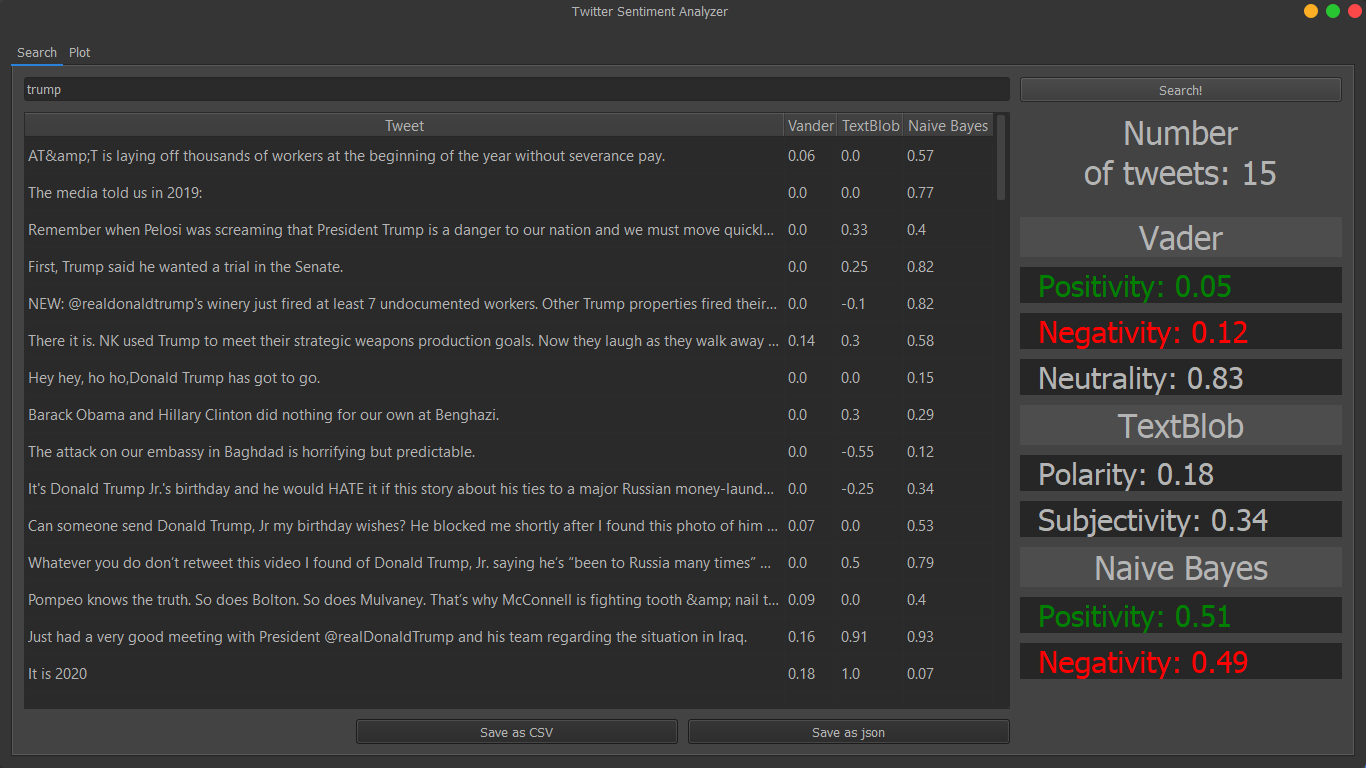
\includegraphics[width=\textwidth]{realisation/assets/1.png}
    \caption{fenêtre de recherche}
    \label{fig:my_label}
\end{figure}
Comme on voit dans la photo ci-dessus, la fenêtre de recherche donne la possibilité au client de:
\begin{itemize}
    \item Entrer un mot ou une phrase et rechercher (en cliquant sur "search") les tweets qui contiennent le texte entré.
    \item Visionner le nombre total et les résultats de ces tweets, les scores de chaque tweet, et le score moyen de tous les tweets selon les différents outils d'analyse de sentiments utilisés.
    \item Enregistrer ses résultats dans le disque dur selon le format choisi (Save as CSV, Save as JSON) 
\end{itemize}
\begin{figure}[H]
    \centering
    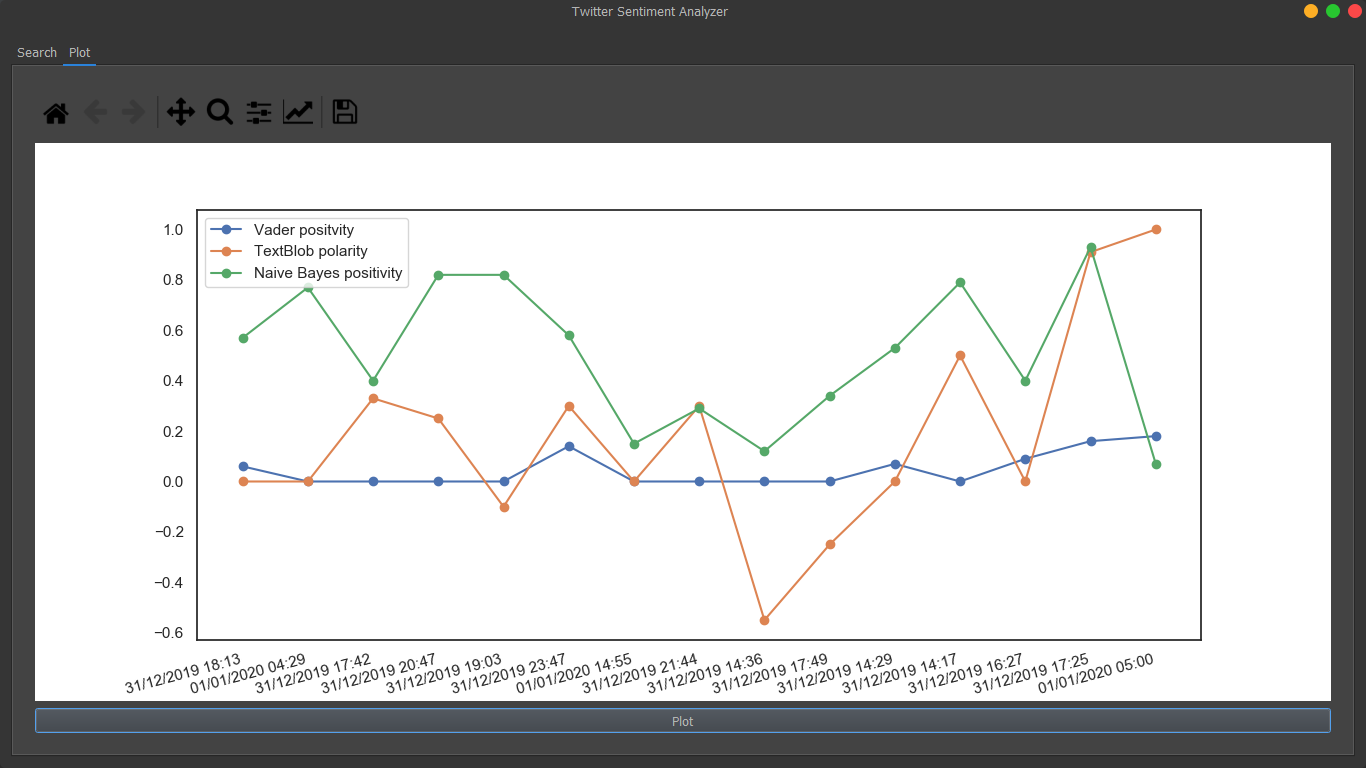
\includegraphics[width=\textwidth]{realisation/assets/2.png}
    \caption{fenêtre de graphe}
    \label{fig:my_label}
\end{figure}
La fenêtre "plot" donne la main au client pour:
\begin{itemize}
    \item Tracer graphiquement (en cliquant sur "plot") les variations de sentiments selon les moyens d'analyse de sentiments présents.
    \item Enregistrer ces graphes dans le disque dur (en cliquant sur l'icone d'enregistrement).
\end{itemize}
\section{Conclusion}
Dans ce chapitre, nous avons détaillé notre implémentation de l'algorithme Bayes Naive, discuté les différentes librairies et APIs choisis pour la réalisation du projet, aussi que les différents écran constituant notre interface graphique.

\chapter{Conclusion}
Dans ce projet, nous devions concevoir et développer une application desktop d'analyse des sentiments des tweets en temps réel.

Dans ce rapport, nous avons commencé par une présentation du contexte générale du projet, comme on a examiné l'étude théorique effectuée lors de la réalisation en abordant l'aspect conceptuel du projet, on a aussi discuté les différents choix techniques qui nous ont aidé à l'élaboration de notre application, avant de détailler les différentes étapes de l'implémentation du projet.

La démarche utilisée pour résoudre ce problème a tout de même quelques limites qui malheureusement demande plus de temps et de moyen afin de les aborder, on peut citer comme exemple le nombre des tweets fournis par TwitterAPI, qui se limite à x tweet, ainsi les humains peuvent exprimer leurs émotions de manière déguisée sans utiliser de vocabulaire émotif. Par exemple, "Mon travail m'oblige à travailler 25 heures par jour". Bien sûr, dans cette phrase, le locuteur exprime un sentiment négatif hyperbolique, suggérant qu'il doit travailler trop pour son travail. De telles expressions ne peuvent être saisies qu'à l'aide d'une base de connaissances du monde réel. En plus, la complexité des langues humains (anglaise dans notre cas) nous empêche à détecter très précisément les sentiments des tweets étudiés.

Dans les versions futures, Nous pourrions encore améliorer notre application en essayant d'extraire plus de fonctionnalités des tweets, en essayant différents types de fonctionnalités, en ajustant les paramètres du classificateur naïf de Bayes, ou en essayant un autre classificateur tous ensemble.

\bibliography{bibliography}{}
\bibliographystyle{apalike}

\begin{appendices}
    \chapter{Formation de notre modèle Naive Bayes pour l'analyse des sentiments sur Twitter}
\label{naivebayesimplementation}
\begin{tcolorbox}[breakable, size=fbox, boxrule=1pt, pad at break*=1mm,colback=cellbackground, colframe=cellborder]
    \prompt{In}{incolor}{20}{\boxspacing}
    \begin{Verbatim}[commandchars=\\\{\}]
        \PY{k+kn}{import} \PY{n+nn}{pandas} \PY{k}{as} \PY{n+nn}{pd}
        \PY{k+kn}{import} \PY{n+nn}{numpy} \PY{k}{as} \PY{n+nn}{np}
        \PY{k+kn}{import} \PY{n+nn}{nltk}
        \PY{n}{nltk}\PY{o}{.}\PY{n}{download}\PY{p}{(}\PY{l+s+s1}{\PYZsq{}}\PY{l+s+s1}{stopwords}\PY{l+s+s1}{\PYZsq{}}\PY{p}{)}
        \PY{n}{nltk}\PY{o}{.}\PY{n}{download}\PY{p}{(}\PY{l+s+s1}{\PYZsq{}}\PY{l+s+s1}{punkt}\PY{l+s+s1}{\PYZsq{}}\PY{p}{)}
    \end{Verbatim}
\end{tcolorbox}

\begin{Verbatim}[commandchars=\\\{\}]
    [nltk\_data] Downloading package stopwords to /root/nltk\_data{\ldots}
    [nltk\_data]   Package stopwords is already up-to-date!
    [nltk\_data] Downloading package punkt to /root/nltk\_data{\ldots}
    [nltk\_data]   Package punkt is already up-to-date!
\end{Verbatim}

\begin{tcolorbox}[breakable, size=fbox, boxrule=.5pt, pad at break*=1mm, opacityfill=0]
    \prompt{Out}{outcolor}{20}{\boxspacing}
    \begin{Verbatim}[commandchars=\\\{\}]
        True
    \end{Verbatim}
\end{tcolorbox}

\begin{tcolorbox}[breakable, size=fbox, boxrule=1pt, pad at break*=1mm,colback=cellbackground, colframe=cellborder]
    \prompt{In}{incolor}{21}{\boxspacing}
    \begin{Verbatim}[commandchars=\\\{\}]
        \PY{k+kn}{from} \PY{n+nn}{google}\PY{n+nn}{.}\PY{n+nn}{colab} \PY{k}{import} \PY{n}{drive}
        \PY{n}{drive}\PY{o}{.}\PY{n}{mount}\PY{p}{(}\PY{l+s+s1}{\PYZsq{}}\PY{l+s+s1}{/content/drive}\PY{l+s+s1}{\PYZsq{}}\PY{p}{)}
    \end{Verbatim}
\end{tcolorbox}

\begin{Verbatim}[commandchars=\\\{\}]
    Drive already mounted at /content/drive; to attempt to forcibly remount, call
    drive.mount("/content/drive", force\_remount=True).
\end{Verbatim}

\begin{tcolorbox}[breakable, size=fbox, boxrule=1pt, pad at break*=1mm,colback=cellbackground, colframe=cellborder]
    \prompt{In}{incolor}{22}{\boxspacing}
    \begin{Verbatim}[commandchars=\\\{\}]
        \PY{n}{tweets} \PY{o}{=} \PY{n}{pd}\PY{o}{.}\PY{n}{read\PYZus{}csv}\PY{p}{(}\PY{l+s+s2}{\PYZdq{}}\PY{l+s+s2}{/content/drive/My Drive/Colab Notebooks/Tweets/tweets.csv}\PY{l+s+s2}{\PYZdq{}}\PY{p}{,} \PY{n}{header} \PY{o}{=} \PY{k+kc}{None}\PY{p}{,} \PY{n}{names}\PY{o}{=}\PY{p}{[}\PY{l+s+s2}{\PYZdq{}}\PY{l+s+s2}{score}\PY{l+s+s2}{\PYZdq{}}\PY{p}{,} \PY{l+s+s2}{\PYZdq{}}\PY{l+s+s2}{text}\PY{l+s+s2}{\PYZdq{}}\PY{p}{]}\PY{p}{)}\PY{o}{.}\PY{n}{drop}\PY{p}{(}\PY{l+m+mi}{0}\PY{p}{)}
        \PY{n}{tweets}\PY{o}{.}\PY{n}{head}\PY{p}{(}\PY{p}{)}
    \end{Verbatim}
\end{tcolorbox}

\begin{Verbatim}[commandchars=\\\{\}]
    /usr/local/lib/python3.6/dist-packages/IPython/core/interactiveshell.py:2718:
    DtypeWarning: Columns (0) have mixed types. Specify dtype option on import or
    set low\_memory=False.
    interactivity=interactivity, compiler=compiler, result=result)
\end{Verbatim}

\begin{tcolorbox}[breakable, size=fbox, boxrule=.5pt, pad at break*=1mm, opacityfill=0]
    \prompt{Out}{outcolor}{22}{\boxspacing}
    \begin{Verbatim}[commandchars=\\\{\}]
        score                                               text
        1     0  @switchfoot http://twitpic.com/2y1zl - Awww, t{\ldots}
        2     0  is upset that he can't update his Facebook by {\ldots}
        3     0  @Kenichan I dived many times for the ball. Man{\ldots}
        4     0    my whole body feels itchy and like its on fire
        5     0  @nationwideclass no, it's not behaving at all{\ldots}
    \end{Verbatim}
\end{tcolorbox}

\begin{tcolorbox}[breakable, size=fbox, boxrule=1pt, pad at break*=1mm,colback=cellbackground, colframe=cellborder]
    \prompt{In}{incolor}{0}{\boxspacing}
    \begin{Verbatim}[commandchars=\\\{\}]
        \PY{k+kn}{from} \PY{n+nn}{sklearn}\PY{n+nn}{.}\PY{n+nn}{utils} \PY{k}{import} \PY{n}{shuffle}

        \PY{n}{tweets} \PY{o}{=} \PY{n}{shuffle}\PY{p}{(}\PY{n}{tweets}\PY{p}{)}
    \end{Verbatim}
\end{tcolorbox}

\begin{tcolorbox}[breakable, size=fbox, boxrule=1pt, pad at break*=1mm,colback=cellbackground, colframe=cellborder]
    \prompt{In}{incolor}{0}{\boxspacing}
    \begin{Verbatim}[commandchars=\\\{\}]
        \PY{k+kn}{import} \PY{n+nn}{re}
        \PY{k+kn}{from} \PY{n+nn}{nltk}\PY{n+nn}{.}\PY{n+nn}{tokenize} \PY{k}{import} \PY{n}{word\PYZus{}tokenize}
        \PY{k+kn}{from} \PY{n+nn}{string} \PY{k}{import} \PY{n}{punctuation}
        \PY{k+kn}{from} \PY{n+nn}{nltk}\PY{n+nn}{.}\PY{n+nn}{corpus} \PY{k}{import} \PY{n}{stopwords}

        \PY{k}{class} \PY{n+nc}{PreProcessTweets}\PY{p}{:}
        \PY{k}{def} \PY{n+nf}{\PYZus{}\PYZus{}init\PYZus{}\PYZus{}}\PY{p}{(}\PY{n+nb+bp}{self}\PY{p}{)}\PY{p}{:}
        \PY{n+nb+bp}{self}\PY{o}{.}\PY{n}{\PYZus{}stopwords} \PY{o}{=} \PY{n+nb}{set}\PY{p}{(}\PY{n}{stopwords}\PY{o}{.}\PY{n}{words}\PY{p}{(}\PY{l+s+s1}{\PYZsq{}}\PY{l+s+s1}{english}\PY{l+s+s1}{\PYZsq{}}\PY{p}{)} \PY{o}{+} \PY{n+nb}{list}\PY{p}{(}\PY{n}{punctuation}\PY{p}{)} \PY{o}{+} \PY{p}{[}\PY{l+s+s1}{\PYZsq{}}\PY{l+s+s1}{AT\PYZus{}USER}\PY{l+s+s1}{\PYZsq{}}\PY{p}{,} \PY{l+s+s1}{\PYZsq{}}\PY{l+s+s1}{URL}\PY{l+s+s1}{\PYZsq{}}\PY{p}{]}\PY{p}{)}

        \PY{k}{def} \PY{n+nf}{process\PYZus{}tweets}\PY{p}{(}\PY{n+nb+bp}{self}\PY{p}{,} \PY{n}{list\PYZus{}of\PYZus{}tweets}\PY{p}{)}\PY{p}{:}
        \PY{n}{processed\PYZus{}tweets} \PY{o}{=} \PY{p}{[}\PY{p}{]}
        \PY{k}{for} \PY{n}{index}\PY{p}{,} \PY{n}{tweet} \PY{o+ow}{in} \PY{n}{list\PYZus{}of\PYZus{}tweets}\PY{o}{.}\PY{n}{iterrows}\PY{p}{(}\PY{p}{)}\PY{p}{:}
        \PY{n}{processed\PYZus{}tweets}\PY{o}{.}\PY{n}{append}\PY{p}{(}\PY{p}{(}\PY{n+nb+bp}{self}\PY{o}{.}\PY{n}{\PYZus{}process\PYZus{}tweet}\PY{p}{(}\PY{n}{tweet}\PY{p}{[}\PY{l+s+s2}{\PYZdq{}}\PY{l+s+s2}{text}\PY{l+s+s2}{\PYZdq{}}\PY{p}{]}\PY{p}{)}\PY{p}{,} \PY{n}{tweet}\PY{p}{[}\PY{l+s+s2}{\PYZdq{}}\PY{l+s+s2}{score}\PY{l+s+s2}{\PYZdq{}}\PY{p}{]}\PY{p}{)}\PY{p}{)}
        \PY{k}{return} \PY{n}{processed\PYZus{}tweets}

        \PY{k}{def} \PY{n+nf}{\PYZus{}process\PYZus{}tweet}\PY{p}{(}\PY{n+nb+bp}{self}\PY{p}{,} \PY{n}{tweet}\PY{p}{)}\PY{p}{:}
        \PY{n}{tweet} \PY{o}{=} \PY{n}{tweet}\PY{o}{.}\PY{n}{lower}\PY{p}{(}\PY{p}{)}  \PY{c+c1}{\PYZsh{} convert text to lower\PYZhy{}case}
        \PY{n}{tweet} \PY{o}{=} \PY{n}{re}\PY{o}{.}\PY{n}{sub}\PY{p}{(}\PY{l+s+sa}{r}\PY{l+s+s1}{\PYZsq{}}\PY{l+s+s1}{((www}\PY{l+s+s1}{\PYZbs{}}\PY{l+s+s1}{.[\PYZca{}}\PY{l+s+s1}{\PYZbs{}}\PY{l+s+s1}{s]+)|(https?://[\PYZca{}}\PY{l+s+s1}{\PYZbs{}}\PY{l+s+s1}{s]+))}\PY{l+s+s1}{\PYZsq{}}\PY{p}{,} \PY{l+s+s1}{\PYZsq{}}\PY{l+s+s1}{URL}\PY{l+s+s1}{\PYZsq{}}\PY{p}{,} \PY{n}{tweet}\PY{p}{)}  \PY{c+c1}{\PYZsh{} remove URLs}
        \PY{n}{tweet} \PY{o}{=} \PY{n}{re}\PY{o}{.}\PY{n}{sub}\PY{p}{(}\PY{l+s+sa}{r}\PY{l+s+s1}{\PYZsq{}}\PY{l+s+s1}{@[\PYZca{}}\PY{l+s+s1}{\PYZbs{}}\PY{l+s+s1}{s]+}\PY{l+s+s1}{\PYZsq{}}\PY{p}{,} \PY{l+s+s1}{\PYZsq{}}\PY{l+s+s1}{AT\PYZus{}USER}\PY{l+s+s1}{\PYZsq{}}\PY{p}{,} \PY{n}{tweet}\PY{p}{)}  \PY{c+c1}{\PYZsh{} remove usernames}
        \PY{n}{tweet} \PY{o}{=} \PY{n}{re}\PY{o}{.}\PY{n}{sub}\PY{p}{(}\PY{l+s+sa}{r}\PY{l+s+s1}{\PYZsq{}}\PY{l+s+s1}{\PYZsh{}([\PYZca{}}\PY{l+s+s1}{\PYZbs{}}\PY{l+s+s1}{s]+)}\PY{l+s+s1}{\PYZsq{}}\PY{p}{,} \PY{l+s+sa}{r}\PY{l+s+s1}{\PYZsq{}}\PY{l+s+s1}{\PYZbs{}}\PY{l+s+s1}{1}\PY{l+s+s1}{\PYZsq{}}\PY{p}{,} \PY{n}{tweet}\PY{p}{)}  \PY{c+c1}{\PYZsh{} remove the \PYZsh{} in \PYZsh{}hashtag}
        \PY{n}{tweet} \PY{o}{=} \PY{n}{word\PYZus{}tokenize}\PY{p}{(}\PY{n}{tweet}\PY{p}{)}  \PY{c+c1}{\PYZsh{} remove repeated characters}
        \PY{k}{return} \PY{p}{[}\PY{n}{word} \PY{k}{for} \PY{n}{word} \PY{o+ow}{in} \PY{n}{tweet} \PY{k}{if} \PY{n}{word} \PY{o+ow}{not} \PY{o+ow}{in} \PY{n+nb+bp}{self}\PY{o}{.}\PY{n}{\PYZus{}stopwords}\PY{p}{]}
    \end{Verbatim}
\end{tcolorbox}
d
\begin{tcolorbox}[breakable, size=fbox, boxrule=1pt, pad at break*=1mm,colback=cellbackground, colframe=cellborder]
    \prompt{In}{incolor}{0}{\boxspacing}
    \begin{Verbatim}[commandchars=\\\{\}]
        \PY{n}{processor} \PY{o}{=} \PY{n}{PreProcessTweets}\PY{p}{(}\PY{p}{)}
        \PY{n}{processed\PYZus{}tweets} \PY{o}{=} \PY{n}{processor}\PY{o}{.}\PY{n}{process\PYZus{}tweets}\PY{p}{(}\PY{n}{tweets}\PY{o}{.}\PY{n}{head}\PY{p}{(}\PY{l+m+mi}{50000}\PY{p}{)}\PY{p}{)}
    \end{Verbatim}
\end{tcolorbox}

\begin{tcolorbox}[breakable, size=fbox, boxrule=1pt, pad at break*=1mm,colback=cellbackground, colframe=cellborder]
    \prompt{In}{incolor}{0}{\boxspacing}
    \begin{Verbatim}[commandchars=\\\{\}]
        \PY{n}{index} \PY{o}{=} \PY{n+nb}{int}\PY{p}{(}\PY{n}{np}\PY{o}{.}\PY{n}{ceil}\PY{p}{(}\PY{n+nb}{len}\PY{p}{(}\PY{n}{processed\PYZus{}tweets}\PY{p}{)} \PY{o}{*} \PY{l+m+mf}{0.8}\PY{p}{)}\PY{p}{)}

        \PY{n}{train} \PY{o}{=} \PY{n}{processed\PYZus{}tweets}\PY{p}{[}\PY{p}{:}\PY{n}{index}\PY{p}{]}
        \PY{n}{test} \PY{o}{=} \PY{n}{processed\PYZus{}tweets}\PY{p}{[}\PY{n}{index}\PY{p}{:}\PY{p}{]}
    \end{Verbatim}
\end{tcolorbox}

\begin{tcolorbox}[breakable, size=fbox, boxrule=1pt, pad at break*=1mm,colback=cellbackground, colframe=cellborder]
    \prompt{In}{incolor}{0}{\boxspacing}
    \begin{Verbatim}[commandchars=\\\{\}]
        \PY{k}{def} \PY{n+nf}{build\PYZus{}vocabulary}\PY{p}{(}\PY{n}{preprocessed\PYZus{}training\PYZus{}data}\PY{p}{)}\PY{p}{:}
        \PY{n}{all\PYZus{}words} \PY{o}{=} \PY{p}{[}\PY{p}{]}

        \PY{k}{for} \PY{p}{(}\PY{n}{words}\PY{p}{,} \PY{n}{\PYZus{}}\PY{p}{)} \PY{o+ow}{in} \PY{n}{preprocessed\PYZus{}training\PYZus{}data}\PY{p}{:}
        \PY{n}{all\PYZus{}words}\PY{o}{.}\PY{n}{extend}\PY{p}{(}\PY{n}{words}\PY{p}{)}

        \PY{n}{word\PYZus{}list} \PY{o}{=} \PY{n}{nltk}\PY{o}{.}\PY{n}{FreqDist}\PY{p}{(}\PY{n}{all\PYZus{}words}\PY{p}{)}
        \PY{n}{word\PYZus{}features} \PY{o}{=} \PY{n}{word\PYZus{}list}\PY{o}{.}\PY{n}{keys}\PY{p}{(}\PY{p}{)}

        \PY{k}{return} \PY{n}{word\PYZus{}features}
    \end{Verbatim}
\end{tcolorbox}

\begin{tcolorbox}[breakable, size=fbox, boxrule=1pt, pad at break*=1mm,colback=cellbackground, colframe=cellborder]
    \prompt{In}{incolor}{0}{\boxspacing}
    \begin{Verbatim}[commandchars=\\\{\}]
        \PY{k}{class} \PY{n+nc}{NaiveBayesModel}\PY{p}{:}
        \PY{k}{def} \PY{n+nf}{\PYZus{}\PYZus{}init\PYZus{}\PYZus{}}\PY{p}{(}\PY{n+nb+bp}{self}\PY{p}{,} \PY{n}{preprocessed\PYZus{}set}\PY{p}{)}\PY{p}{:}
        \PY{n+nb+bp}{self}\PY{o}{.}\PY{n}{word\PYZus{}features} \PY{o}{=} \PY{k+kc}{None}
        \PY{n+nb+bp}{self}\PY{o}{.}\PY{n}{preprocessed\PYZus{}set} \PY{o}{=} \PY{n}{preprocessed\PYZus{}set}
        \PY{n+nb+bp}{self}\PY{o}{.}\PY{n}{classifier} \PY{o}{=} \PY{k+kc}{None}

        \PY{k}{def} \PY{n+nf}{save}\PY{p}{(}\PY{n+nb+bp}{self}\PY{p}{)}\PY{p}{:}
        \PY{k}{with} \PY{n+nb}{open}\PY{p}{(}\PY{l+s+s1}{\PYZsq{}}\PY{l+s+s1}{/content/drive/My Drive/Colab Notebooks/Tweets/my\PYZus{}naivebayes\PYZus{}classifier.pickle}\PY{l+s+s1}{\PYZsq{}}\PY{p}{,} \PY{l+s+s1}{\PYZsq{}}\PY{l+s+s1}{wb}\PY{l+s+s1}{\PYZsq{}}\PY{p}{)} \PY{k}{as} \PY{n}{file}\PY{p}{:}
        \PY{n}{pickle}\PY{o}{.}\PY{n}{dump}\PY{p}{(}\PY{n+nb+bp}{self}\PY{o}{.}\PY{n}{classifier}\PY{p}{,} \PY{n}{file}\PY{p}{)}
        \PY{n+nb}{print}\PY{p}{(}\PY{l+s+s2}{\PYZdq{}}\PY{l+s+s2}{Model saved.}\PY{l+s+s2}{\PYZdq{}}\PY{p}{)}

        \PY{k}{def} \PY{n+nf}{load}\PY{p}{(}\PY{n+nb+bp}{self}\PY{p}{)}\PY{p}{:}
        \PY{k}{with} \PY{n+nb}{open}\PY{p}{(}\PY{l+s+s1}{\PYZsq{}}\PY{l+s+s1}{/content/drive/My Drive/Colab Notebooks/Tweets/my\PYZus{}naivebayes\PYZus{}classifier.pickle}\PY{l+s+s1}{\PYZsq{}}\PY{p}{,} \PY{l+s+s1}{\PYZsq{}}\PY{l+s+s1}{rb}\PY{l+s+s1}{\PYZsq{}}\PY{p}{)} \PY{k}{as} \PY{n}{file}\PY{p}{:}
        \PY{n+nb+bp}{self}\PY{o}{.}\PY{n}{classifier} \PY{o}{=} \PY{n}{pickle}\PY{o}{.}\PY{n}{load}\PY{p}{(}\PY{n}{file}\PY{p}{)}
        \PY{n+nb}{print}\PY{p}{(}\PY{l+s+s2}{\PYZdq{}}\PY{l+s+s2}{Model loaded.}\PY{l+s+s2}{\PYZdq{}}\PY{p}{)}

        \PY{k}{def} \PY{n+nf}{extract\PYZus{}features}\PY{p}{(}\PY{n+nb+bp}{self}\PY{p}{,} \PY{n}{tweet}\PY{p}{)}\PY{p}{:}
        \PY{n}{tweet\PYZus{}words} \PY{o}{=} \PY{n+nb}{set}\PY{p}{(}\PY{n}{tweet}\PY{p}{)}
        \PY{n}{features} \PY{o}{=} \PY{p}{\PYZob{}}\PY{p}{\PYZcb{}}
        \PY{k}{for} \PY{n}{word} \PY{o+ow}{in} \PY{n+nb+bp}{self}\PY{o}{.}\PY{n}{word\PYZus{}features}\PY{p}{:}
        \PY{n}{features}\PY{p}{[}\PY{l+s+s2}{\PYZdq{}}\PY{l+s+si}{\PYZob{}\PYZcb{}}\PY{l+s+s2}{\PYZdq{}}\PY{o}{.}\PY{n}{format}\PY{p}{(}\PY{n}{word}\PY{p}{)}\PY{p}{]} \PY{o}{=} \PY{p}{(}\PY{n}{word} \PY{o+ow}{in} \PY{n}{tweet\PYZus{}words}\PY{p}{)}
        \PY{k}{return} \PY{n}{features}

        \PY{k}{def} \PY{n+nf}{result\PYZus{}labels}\PY{p}{(}\PY{n+nb+bp}{self}\PY{p}{,} \PY{n}{test\PYZus{}set}\PY{p}{)}\PY{p}{:}
        \PY{k}{if} \PY{n+nb+bp}{self}\PY{o}{.}\PY{n}{classifier} \PY{o+ow}{is} \PY{o+ow}{not} \PY{k+kc}{None}\PY{p}{:}
        \PY{n}{labels} \PY{o}{=} \PY{p}{[}\PY{n+nb+bp}{self}\PY{o}{.}\PY{n}{classifier}\PY{o}{.}\PY{n}{classify}\PY{p}{(}\PY{n+nb+bp}{self}\PY{o}{.}\PY{n}{extract\PYZus{}features}\PY{p}{(}\PY{n}{tweet}\PY{p}{[}\PY{l+m+mi}{0}\PY{p}{]}\PY{p}{)}\PY{p}{)} \PY{k}{for} \PY{n}{tweet} \PY{o+ow}{in} \PY{n}{test\PYZus{}set}\PY{p}{]}
        \PY{k}{return} \PY{l+m+mi}{100} \PY{o}{*} \PY{n}{labels}\PY{o}{.}\PY{n}{count}\PY{p}{(}\PY{l+m+mi}{1}\PY{p}{)} \PY{o}{/} \PY{n+nb}{len}\PY{p}{(}\PY{n}{labels}\PY{p}{)}

        \PY{k}{def} \PY{n+nf}{test\PYZus{}and\PYZus{}print\PYZus{}results}\PY{p}{(}\PY{n+nb+bp}{self}\PY{p}{,} \PY{n}{test\PYZus{}set}\PY{p}{)}\PY{p}{:}
        \PY{n}{lb} \PY{o}{=} \PY{l+m+mi}{0}
        \PY{k}{for} \PY{n}{text}\PY{p}{,} \PY{n}{score} \PY{o+ow}{in} \PY{n}{test\PYZus{}set}\PY{p}{:}
        \PY{k}{if} \PY{n}{score} \PY{o}{==} \PY{l+m+mi}{1}\PY{p}{:}
        \PY{n}{lb} \PY{o}{+}\PY{o}{=} \PY{l+m+mi}{1}
        \PY{n}{real\PYZus{}score} \PY{o}{=} \PY{l+m+mi}{100} \PY{o}{*} \PY{n}{lb} \PY{o}{/} \PY{n+nb}{len}\PY{p}{(}\PY{n}{test\PYZus{}set}\PY{p}{)}
        \PY{n}{predicted\PYZus{}score} \PY{o}{=} \PY{n+nb+bp}{self}\PY{o}{.}\PY{n}{result\PYZus{}labels}\PY{p}{(}\PY{n}{test\PYZus{}set}\PY{p}{)}

        \PY{n+nb}{print}\PY{p}{(}\PY{l+s+s2}{\PYZdq{}}\PY{l+s+s2}{Real score: }\PY{l+s+si}{\PYZob{}\PYZcb{}}\PY{l+s+s2}{\PYZdq{}}\PY{o}{.}\PY{n}{format}\PY{p}{(}\PY{n}{real\PYZus{}score}\PY{p}{)}\PY{p}{)}
        \PY{n+nb}{print}\PY{p}{(}\PY{l+s+s2}{\PYZdq{}}\PY{l+s+s2}{Predicted score: }\PY{l+s+si}{\PYZob{}\PYZcb{}}\PY{l+s+s2}{\PYZdq{}}\PY{o}{.}\PY{n}{format}\PY{p}{(}\PY{n}{predicted\PYZus{}score}\PY{p}{)}\PY{p}{)}

        \PY{k}{def} \PY{n+nf}{train\PYZus{}naive\PYZus{}bayes}\PY{p}{(}\PY{n+nb+bp}{self}\PY{p}{)}\PY{p}{:}
        \PY{n+nb+bp}{self}\PY{o}{.}\PY{n}{word\PYZus{}features} \PY{o}{=} \PY{n}{build\PYZus{}vocabulary}\PY{p}{(}\PY{n+nb+bp}{self}\PY{o}{.}\PY{n}{preprocessed\PYZus{}set}\PY{p}{)}
        \PY{n}{training\PYZus{}features} \PY{o}{=} \PY{n}{nltk}\PY{o}{.}\PY{n}{classify}\PY{o}{.}\PY{n}{apply\PYZus{}features}\PY{p}{(}\PY{n+nb+bp}{self}\PY{o}{.}\PY{n}{extract\PYZus{}features}\PY{p}{,} \PY{n+nb+bp}{self}\PY{o}{.}\PY{n}{preprocessed\PYZus{}set}\PY{p}{)}
        \PY{n+nb+bp}{self}\PY{o}{.}\PY{n}{classifier} \PY{o}{=} \PY{n}{nltk}\PY{o}{.}\PY{n}{NaiveBayesClassifier}\PY{o}{.}\PY{n}{train}\PY{p}{(}\PY{n}{training\PYZus{}features}\PY{p}{)}
    \end{Verbatim}
\end{tcolorbox}

\begin{tcolorbox}[breakable, size=fbox, boxrule=1pt, pad at break*=1mm,colback=cellbackground, colframe=cellborder]
    \prompt{In}{incolor}{0}{\boxspacing}
    \begin{Verbatim}[commandchars=\\\{\}]
        \PY{n}{nb} \PY{o}{=} \PY{n}{NaiveBayesModel}\PY{p}{(}\PY{n}{train}\PY{p}{)}
    \end{Verbatim}
\end{tcolorbox}

\begin{tcolorbox}[breakable, size=fbox, boxrule=1pt, pad at break*=1mm,colback=cellbackground, colframe=cellborder]
    \prompt{In}{incolor}{0}{\boxspacing}
    \begin{Verbatim}[commandchars=\\\{\}]
        \PY{n}{nb}\PY{o}{.}\PY{n}{train\PYZus{}naive\PYZus{}bayes}\PY{p}{(}\PY{p}{)}
    \end{Verbatim}
\end{tcolorbox}

\begin{tcolorbox}[breakable, size=fbox, boxrule=1pt, pad at break*=1mm,colback=cellbackground, colframe=cellborder]
    \prompt{In}{incolor}{31}{\boxspacing}
    \begin{Verbatim}[commandchars=\\\{\}]
        \PY{n}{nb}\PY{o}{.}\PY{n}{test\PYZus{}and\PYZus{}print\PYZus{}results}\PY{p}{(}\PY{n}{test}\PY{p}{)}
    \end{Verbatim}
\end{tcolorbox}

\begin{Verbatim}[commandchars=\\\{\}]
    Real score: 48.9
    Predicted score: 52.3
\end{Verbatim}

\begin{tcolorbox}[breakable, size=fbox, boxrule=1pt, pad at break*=1mm,colback=cellbackground, colframe=cellborder]
    \prompt{In}{incolor}{32}{\boxspacing}
    \begin{Verbatim}[commandchars=\\\{\}]
        \PY{k+kn}{import} \PY{n+nn}{pickle}
        \PY{n}{nb}\PY{o}{.}\PY{n}{save}\PY{p}{(}\PY{p}{)}
    \end{Verbatim}
\end{tcolorbox}

\begin{Verbatim}[commandchars=\\\{\}]
    Model saved.
\end{Verbatim}

\begin{tcolorbox}[breakable, size=fbox, boxrule=1pt, pad at break*=1mm,colback=cellbackground, colframe=cellborder]
    \prompt{In}{incolor}{0}{\boxspacing}
    \begin{Verbatim}[commandchars=\\\{\}]
        \PY{k+kn}{import} \PY{n+nn}{csv}
        \PY{k}{def} \PY{n+nf}{save\PYZus{}vocabulary}\PY{p}{(}\PY{n}{file\PYZus{}path}\PY{p}{,} \PY{n}{word\PYZus{}list}\PY{p}{)}\PY{p}{:}
        \PY{k}{with} \PY{n+nb}{open}\PY{p}{(}\PY{n}{file\PYZus{}path}\PY{p}{,} \PY{l+s+s1}{\PYZsq{}}\PY{l+s+s1}{w}\PY{l+s+s1}{\PYZsq{}}\PY{p}{,} \PY{n}{newline}\PY{o}{=}\PY{l+s+s1}{\PYZsq{}}\PY{l+s+s1}{\PYZsq{}}\PY{p}{)} \PY{k}{as} \PY{n}{file}\PY{p}{:}
        \PY{n}{writer} \PY{o}{=} \PY{n}{csv}\PY{o}{.}\PY{n}{writer}\PY{p}{(}\PY{n}{file}\PY{p}{)}
        \PY{k}{for} \PY{n}{word} \PY{o+ow}{in} \PY{n}{word\PYZus{}list}\PY{p}{:}
        \PY{n}{writer}\PY{o}{.}\PY{n}{writerow}\PY{p}{(}\PY{p}{[}\PY{n+nb}{str}\PY{p}{(}\PY{n}{word}\PY{p}{)}\PY{p}{]}\PY{p}{)}
        \PY{n+nb}{print}\PY{p}{(}\PY{l+s+s2}{\PYZdq{}}\PY{l+s+s2}{Dictionary saved.}\PY{l+s+s2}{\PYZdq{}}\PY{p}{)}
    \end{Verbatim}
\end{tcolorbox}

\begin{tcolorbox}[breakable, size=fbox, boxrule=1pt, pad at break*=1mm,colback=cellbackground, colframe=cellborder]
    \prompt{In}{incolor}{34}{\boxspacing}
    \begin{Verbatim}[commandchars=\\\{\}]
        \PY{n}{save\PYZus{}vocabulary}\PY{p}{(}\PY{l+s+s2}{\PYZdq{}}\PY{l+s+s2}{/content/drive/My Drive/Colab Notebooks/Tweets/word\PYZus{}features.csv}\PY{l+s+s2}{\PYZdq{}}\PY{p}{,} \PY{n}{nb}\PY{o}{.}\PY{n}{word\PYZus{}features}\PY{p}{)}
    \end{Verbatim}
\end{tcolorbox}

\begin{Verbatim}[commandchars=\\\{\}]
    Dictionary saved.
\end{Verbatim}

\end{appendices}

\end{document}